% ───────────────────────────────────────────────────────────────────────────
% SplitGuard-AD manuscript. Numbers that come from the GPU programme are
% generated into tables/gpu_numbers.tex by scripts/gpu_postprocess.py.
% ───────────────────────────────────────────────────────────────────────────
% Two-column Springer Nature layout in Times New Roman. `iicol` is the class's
% own two-column option, so this stays inside the JIIM template rather than
% borrowing another publisher's. newtx supplies Times for text and maths
% together, which keeps equations in the same face as the prose.
\documentclass[pdflatex,sn-vancouver-num,iicol]{sn-jnl}

% Packages
\usepackage[utf8]{inputenc}
\usepackage{amsmath,amssymb}
% newtx must follow amssymb, and \Bbbk is defined by both; letting it go here
% is the documented way to load them together.
\let\Bbbk\relax
\usepackage{newtxtext,newtxmath}
\usepackage{graphicx}
\usepackage{booktabs}
% Two-column tables. Column spacing is global; the size is declared in each
% table file, including the two that scripts/generate_adni_paper_tables.py
% writes, so regenerating them keeps the appearance uniform.
\setlength{\tabcolsep}{4pt}
% Full-width floats in a two-column layout queue behind one another, which is
% what pushes a caption a page or two past its first citation. Raising the
% fraction of a page that may be given to floats lets more than one land per
% page and keeps captions near the text that cites them.
\renewcommand{\topfraction}{0.9}
\renewcommand{\dbltopfraction}{0.9}
\renewcommand{\bottomfraction}{0.7}
\renewcommand{\floatpagefraction}{0.75}
\renewcommand{\dblfloatpagefraction}{0.75}
\renewcommand{\textfraction}{0.08}
\setcounter{topnumber}{3}
\setcounter{dbltopnumber}{3}
\setcounter{totalnumber}{5}
% \pb is a zero-width break opportunity for long paths. \texttt offers none, so
% in a two-column measure a path like reports/tables/adni/<file>.json runs into
% the margin. It prints nothing and changes no character of the path, which
% matters: tests/test_repo_hygiene.py checks that every path the manuscript
% names is actually shipped, and it strips \pb before matching.
\newcommand{\pb}{\discretionary{}{}{}}
\renewcommand{\arraystretch}{1.08}
\usepackage{array}   % >{...} column modifiers, for ragged narrow columns
\usepackage{multirow}
\usepackage{xcolor}
\usepackage{tikz}
\usetikzlibrary{arrows.meta,positioning,shapes.geometric}
% Figure palette, shared with the matplotlib figures (Wong 2011). Colour
% encodes protocol identity only; everything else is neutral.
\definecolor{protoA}{HTML}{D55E00}
\definecolor{protoB}{HTML}{009E73}
\definecolor{protoC}{HTML}{0072B2}
\usepackage{pgfplots}
\pgfplotsset{compat=1.18}
\usepackage{subcaption}
\graphicspath{{./}}
\usepackage{algorithm}
\usepackage{algpseudocode}

% Float placement: in the original elsarticle 3p layout figures kept
% getting punted to the end. The two-line fix is (a) load the `float`
% package so a placement specifier `[H]` ("place exactly here") becomes
% available, and (b) load `placeins` with the `section` option so a
% `\FloatBarrier` is inserted automatically before every \section{} ---
% no figure can survive past its parent section.
\usepackage{float}
\usepackage[section]{placeins}
% Extend FloatBarrier from \section to \subsection too --- without this,
% an end-of-subsection figure (e.g. Figure 5 closing §6.1) can spill to
% the top of the next subsection's page (e.g. §6.2 territory).
\usepackage{etoolbox}
% A subsection can opt out of its barrier with \global\skipbarriertrue.
% Used only where the barrier would flush a float that no longer fits and
% end the page early, leaving most of it blank.
\newif\ifskipbarrier
\preto\subsection{\ifskipbarrier\global\skipbarrierfalse\else\FloatBarrier\fi}

% Permissive float-parameter set so LaTeX won't refuse to place a
% figure at the top of a page because some internal quota is exceeded.
\renewcommand{\topfraction}{0.92}
\renewcommand{\bottomfraction}{0.80}
\renewcommand{\textfraction}{0.08}
\renewcommand{\floatpagefraction}{0.80}
\setcounter{topnumber}{3}
\setcounter{bottomnumber}{3}
\setcounter{totalnumber}{5}

% Slightly tighter floats so figures sit closer to their references.
\setlength{\textfloatsep}{10pt plus 2.0pt minus 2.0pt}
\setlength{\intextsep}{10pt plus 2.0pt minus 2.0pt}

% Allow LaTeX to widen spacing slightly so \texttt{} filenames don't
% punch out of the right margin in single-column mode.
\sloppy


% ── Macros ────────────────────────────────────────────────────────────────────
\newcommand{\SGA}{\textsc{SplitGuard-AD}}
\newcommand{\ie}{\textit{i.e.},}
\newcommand{\eg}{\textit{e.g.},}
\newcommand{\etal}{\textit{et al.}}
% \gap{} previously coloured inflation-gap numbers red; for the
% submission-ready manuscript we render them in normal text so the
% reader's eye is not steered by colour. The macro is retained so all
% existing call sites keep working; toggle the body to \textcolor{red}{#1}
% for working-draft inspection if desired.
\newcommand{\gap}[1]{#1}

% Numbers produced by the GPU programme, written by
% scripts/gpu_postprocess.py. A number whose run has not completed
% renders as ?? rather than as a stale value.
% Generated by scripts/gpu_postprocess.py. Do not edit by hand.
% \pending marks a number whose run has not completed.
\providecommand{\pending}{\textbf{??}}
\newcommand{\TierOneRandomAUROC}{0.999}
\newcommand{\TierOneFilenameAUROC}{0.793}
\newcommand{\TierOneTrueAUROC}{0.766}
\newcommand{\TierOneGapTotal}{+0.233}
\newcommand{\TierOneGapCI}{[+0.191, +0.270]}
\newcommand{\TierOneGapFilename}{+0.206}
\newcommand{\TierOneGapResidual}{+0.027}
\newcommand{\TierOneShareFilename}{88.6}
\newcommand{\AdniRandomAUROC}{0.947}
\newcommand{\AdniSubjectAUROC}{0.837}
\newcommand{\AdniSafeAUROC}{0.829}
\newcommand{\AdniGapTotal}{+0.118}
\newcommand{\AdniGapCI}{[+0.096, +0.145]}
\newcommand{\AdniHierGap}{+0.118}
\newcommand{\AdniHierCI}{[+0.061, +0.181]}
\newcommand{\AdniGapExactKey}{+0.113}
\newcommand{\AdniDenseGap}{+0.146}
\newcommand{\AdniConvGap}{+0.142}
\newcommand{\AdniNoMtOneGap}{+0.128}
\newcommand{\AdniNoMtOneCI}{[+0.097, +0.159]}
\newcommand{\SizeBalancedGap}{+0.136}
\newcommand{\AdniSubjectPart}{0.110}
\newcommand{\AdniSubjectPartCI}{[+0.086, +0.139]}
\newcommand{\AdniMarginal}{0.008}
\newcommand{\AdniMarginalCI}{[-0.033, +0.042]}
\newcommand{\AdniConvMarginal}{-0.026}
\newcommand{\AdniArmSpread}{0.028}
\newcommand{\OasisRandomAUROC}{0.828}
\newcommand{\OasisSafeAUROC}{0.793}
\newcommand{\OasisGapTotal}{+0.035}
\newcommand{\OasisGapCI}{[+0.009, +0.064]}
\newcommand{\OasisDenseGap}{+0.048}
\newcommand{\VolGapTotal}{+0.235}
\newcommand{\VolGapCI}{[+0.174, +0.298]}
\newcommand{\ProbeLiftImage}{211.7}
\newcommand{\ProbeLiftSession}{204.8}
\newcommand{\ProvScanTenSubject}{35\%}
\newcommand{\ProvScanTenSafe}{18\%}
\newcommand{\ProvParticipantTenSubject}{36\%}
\newcommand{\ComposedTenSubject}{0.043}
\newcommand{\ComposedTenSafe}{0.022}
\newcommand{\ProvSubjectAUROCTen}{0.865}
\newcommand{\ProvSafeAUROCTen}{0.829}
\newcommand{\CardSens}{65.5\%}
\newcommand{\CardSpec}{81.0\%}
\newcommand{\CardBalAcc}{73.2\%}
\newcommand{\CardAUROC}{0.829}
\newcommand{\CardNTest}{165}
\newcommand{\CardPPVPop}{35.6\%}
\newcommand{\CardNPVPop}{93.6\%}
\newcommand{\CardPPVClinic}{83.2\%}
\newcommand{\CardNPVClinic}{62.1\%}
\newcommand{\GpuHours}{14.8}
\newcommand{\DoseSlope}{0.125}
\newcommand{\DoseAtZero}{0.823}
\newcommand{\DoseDenseAtZero}{0.861}
\newcommand{\DoseDenseSlope}{0.091}
\newcommand{\DoseAtOne}{0.948}
\newcommand{\AdniConvRandomAUROC}{0.957}
\newcommand{\AdniConvSafeAUROC}{0.815}
\newcommand{\DoseIntercept}{0.823}
\newcommand{\DoseRSq}{0.853}
\newcommand{\SensLeaky}{0.866}
\newcommand{\SensSafe}{0.535}
\newcommand{\MissedPerThousand}{45.7}
\newcommand{\AdniShareSubject}{93}


% As in Springer's own sn-article sample: let a short page stay short rather
% than overfill the block.
\raggedbottom

\begin{document}


% ── Title ─────────────────────────────────────────────────────────────────────
\title[Patient Leakage Under Degraded Provenance in AD MRI]{Patient Leakage
       Under Degraded Data Provenance in Alzheimer's Disease MRI Deep
       Learning: Controlled Experiments and the SplitGuard-AD Audit}

% ── Authors ───────────────────────────────────────────────────────────────────
% Affiliation order: Medipol School of Medicine (a), Medipol Engineering (b),
% ETH Zurich (c) — Medipol grouped first because the corresponding author
% holds a dual home-institution appointment (Medicine + Engineering).
\author*[1,2]{\fnm{Mehmet Berke} \sur{Isler}}\email{mehmetberkeisler@gmail.com}

\author[3]{\fnm{Irem} \sur{Ilter}}\email{ilteri@student.ethz.ch}

\author[2]{\fnm{Mehmet Kemal} \sur{Ozdemir}}\email{mkozdemir@medipol.edu.tr}

\affil*[1]{\orgdiv{International School of Medicine},
           \orgname{Istanbul Medipol University},
           \orgaddress{\city{Istanbul}, \country{Türkiye}}}

\affil[2]{\orgdiv{Department of Computer Engineering, School of Engineering
          and Natural Sciences}, \orgname{Istanbul Medipol University},
          \orgaddress{\city{Istanbul}, \country{Türkiye}}}

\affil[3]{\orgdiv{Institute of Neuroinformatics},
          \orgname{ETH Zurich and University of Zurich},
          \orgaddress{\city{Zurich}, \country{Switzerland}}}

% ── Abstract ──────────────────────────────────────────────────────────────────
\abstract{Deep-learning models for Alzheimer's disease (AD) classification from
structural MRI routinely report near-perfect benchmark performance that
does not survive patient-independent evaluation. Splitting by patient
assumes the provenance defining patient identity is complete and correct,
which redistribution and metadata loss routinely violate. We ask how
patient-independent evaluation behaves when it degrades. On ADNI1
($220$ cognitively normal and AD participants, $1{,}123$ scans, one 2D
coronal-centre slice per scan), a random-split area under the receiver
operating characteristic curve (AUROC) of \AdniRandomAUROC{} falls to
\AdniSafeAUROC{} under component-safe evaluation: an inflation gap of
\AdniGapTotal{} \AdniGapCI{}, replicated on OASIS-1 (\OasisGapTotal{}) and
under DenseNet-121. Three controlled experiments separate the links.
Permuting diagnosis labels across participants breaks the systematic
participant-level association between diagnosis and anatomy, yet random
splitting still reaches $0.878$ AUROC while both patient-aware protocols
sit at chance: the apparent skill is patient recall. Substituting training scans
into the test set raises AUROC by $+\DoseSlope{}$ per unit nominal overlap,
descriptive of that procedure, not a causal price. Deleting participant identifiers shows
that a leakage graph prevents $49\%$ of the leakage subject-wise splitting
admits at $10\%$ loss. One case is observed, not simulated: by content
matching, a widely used public 2D AD benchmark redistributes $200$ OASIS-1
participants whose identifiers became a filename index that merges and
splits them, and grouping by it still leaves $70\%$ of test images sharing
a participant with training. Patient independence depends
on both the splitting procedure and the integrity of the provenance
defining patient identity. Manifests, audit code and the rebuild pipeline
are released under Apache-2.0.
}

% ── Keywords ──────────────────────────────────────────────────────────────────
% Target venue is the Journal of Imaging Informatics in Medicine
% (Springer/SIIM), which does not use the Elsevier Highlights convention.
% The former SplitGuard-AD_Highlights.txt is retired to archive/.
% JIIM asks for 4-6 keywords; six are given below.
\keywords{Patient-identity leakage, Evaluation protocol,
          Alzheimer's disease, Structural MRI, Data provenance,
          Reproducibility}

\maketitle


% ══════════════════════════════════════════════════════════════════════════════
\section{Introduction}
\label{sec:intro}
% ══════════════════════════════════════════════════════════════════════════════

Alzheimer's disease (AD) is the leading cause of dementia
worldwide~\cite{who2023} and, under the NIA-AA diagnostic
framework~\cite{jack2011}, a major target for medical-imaging deep
learning. The
modelling literature is mature: 3D residual networks~\cite{korolev2017residual}, hierarchical fully-convolutional
architectures that jointly localise atrophy and
classify~\cite{lian2020hierarchical}, and interpretability-aware
frameworks validated against neuropathology~\cite{qiu2020explainable}.
Reported benchmark accuracy on structural MRI is routinely
near-perfect: a recent scoping review of $44$ AD deep-learning studies
finds a $19$-point accuracy gradient between studies judged at low and
at high risk of leakage~\cite{diagnostics2025}. These reports,
however, rarely survive patient-independent evaluations. One important
cause is \emph{patient-identity leakage} across train and test
partitions. It arises in AD MRI through four channels
(Figure~\ref{fig:leakage_modes}): slices of one 3D volume distributed across
partitions; different visits from one longitudinal record; near-duplicate or
augmentation-derived images on opposite sides of a split; and rescans of the
same session. Because AD MRI research routinely uses longitudinal
cohorts with multiple visits per patient (ADNI: median $5$
scans/subject) as well as slice-based 2D representations, each of
these channels is a live risk in practice. Under any of them, the
trained model recognises images from patients it has already
analysed rather than generalising to new
patients~\cite{wen2020,yagis2021,diagnostics2025}.

That leakage inflates reported performance is established. The evidence
includes slice-wise against subject-wise splitting on four
cohorts~\cite{yagis2021}, a review recommending subject-level
partitioning~\cite{wen2020}, five leakage forms manipulated in connectome
models~\cite{rosenblatt2024}, and a $19$-point accuracy gradient between
studies at low and high risk of leakage in a scoping review of
$44$~\cite{diagnostics2025}.

Why \emph{patient identity} is a particularly important shortcut channel
in longitudinal structural MRI is equally well established. Shortcut learning~\cite{geirhos2020shortcut} exploits
stable but clinically irrelevant cues correlated with the label, as
with hospital-system markers in chest radiographs~\cite{zech2018variable},
non-lung cues in COVID classifiers~\cite{degrave2021shortcuts} and
hidden subgroup failures~\cite{oakden2020hidden}. Structural MRI is
unusually exposed to the identity version: face recognition
re-identifies anonymised scans~\cite{schwarz2019face}, \emph{BrainPrint}
is a stable per-subject fingerprint~\cite{wachinger2015brainprint},
learned representations support cross-cohort subject
re-identification~\cite{deepbrainprint2023}, and even brain-age
prediction carries subject-specific structural
signal~\cite{liem2017brainage}. A model evaluated on subject-leaky data
can therefore appear to recognise disease while partly recognising the
patient, a protocol-driven reliability gap also documented in COVID
imaging~\cite{roberts2021pitfalls}, in medical-imaging machine learning
generally~\cite{varoquaux2022failures}, and as a cross-disciplinary
leakage taxonomy~\cite{kapoor2023leakage}.

The remedy is likewise available: subject-aware splitting ships in
general-purpose libraries (\texttt{GroupKFold}~\cite{pedregosa2011sklearn})
and medical-imaging frameworks (MONAI~\cite{cardoso2022monai}), a
similarity-aware splitter has been proposed~\cite{datasail2025}, and
CLAIM~\cite{claim2024,mongan2020claim}, TRIPOD+AI~\cite{tripod2024} and
PROBAST~\cite{wolff2019probast} all require subject-level splitting for
a low risk-of-bias verdict. Protocol~B groups by \texttt{subject\_id},
the key those guidelines prescribe, though it is this paper's own
participant-wise splitter rather than \texttt{GroupKFold} itself
(\S\ref{sec:exp3_degrad}).

What these studies leave unmeasured is how evaluation optimism changes
with leakage magnitude, and how provenance degradation determines the
leakage that survives a patient-aware split.
Two quantities govern how much optimism a benchmark reports, and
neither has been characterised. The first is how much optimism a unit
of leakage buys. Rosenblatt et al.\ come closest, reporting
performance deltas at three discrete levels of subject repetition
($5$, $10$ and $20\%$) in connectome models, but they fit no function
across those levels and state no per-unit rate. The second has not
been asked at all: what determines how much leakage a given benchmark
admits in the first place. That is a question about data provenance.
A splitting protocol can only keep a patient's images together if the
identifiers it depends on are present and correct; curated research
cohorts supply them, and the redistributed benchmarks the field
actually trains on frequently do not.

In this work we measure both quantities on a single cohort, using one
experimental template for each: hold everything fixed, sweep one
controlled quantity, and read off the curve.

We measure both links of that chain on a single cohort in one code
state, manipulating the two quantities independently. Provenance
integrity is varied by deleting participant identifiers at controlled
rates, and by corrupting them in the two ways redistribution actually
corrupts them: dealing one participant across several keys, and merging
several under one. Test-set contamination is varied separately, by
substituting a measured share of test scans with other scans of
training participants, which also removes those scans from training. A participant-label
permutation serves as the positive control: with the association between
anatomy and diagnosis destroyed, any discrimination a protocol retains
is patient recall and nothing else. One case is observed rather than
imposed, in a widely used public benchmark that redistributes a research
cohort under an identifier that merges and splits its participants.

This paper makes three contributions. First, it shows that
patient-independent evaluation has an untested dependency on provenance
integrity, and quantifies how much leakage survives a patient-aware
protocol as that provenance is degraded and corrupted. Second, it
calibrates what the surviving leakage is worth, through a contamination
dose-response and a permutation control that separates patient recall
from disease signal. Third, it releases \SGA{}, an executable audit that
builds a per-image leakage graph from whatever identifier evidence a
cohort carries, emits a frozen component-safe partition and reports a
pre-training decision, together with the manifests, component tables and
rebuild pipeline behind every number reported here. Where participant
identity is intact the audit's component layer reduces to participant
grouping, and we report that equivalence as a result rather than
defending it as a feature.

The observation that random image-level splits inflate AD MRI scores
is not new by itself. Wen \etal~\cite{wen2020} and Yagis \etal~\cite{yagis2021} quantified the
inflation on individual datasets. Rumala~\cite{rumala2023} showed on
longitudinal brain MRI that folds which do not separate subjects inflate 3D
CNN estimates, and used saliency maps to argue that the network attends to
subject identity. Ghiasi \etal~\cite{ghiasi2026} established a leakage-free
longitudinal dementia benchmark by withholding the label-defining clinical
score and splitting group-aware, reporting the inflated and clean conditions
as an on/off pair. Subject-aware splitting tools such as
DataSAIL~\cite{datasail2025} are available for biomedical data. Separately,
biometric work on MRI
representations~\cite{deepbrainprint2023,wachinger2015brainprint,schwarz2019face}
has established that structural MRI
leaks subject identity at re-identification accuracies far above chance.
Across all of it, leakage is treated as a binary hazard: either the
split respects patients or it does not, and the remedy is to group by
subject. That framing presumes what it needs, a subject identifier
that is present, complete and correct, which is the presumption this
paper measures. Supplementary Table~S4 places the present work
against that literature on the axes that separate them.


The cross-tier inflation gap is validated on two source cohorts and
one redistribution of one of them; the
ADNI-specific findings (subject-level aggregation, sex disparity,
clinical cost, dose-response) are single-cohort findings on ADNI1
itself, and external-cohort replication
(AIBL~\cite{ellis2009aibl}, UK Biobank~\cite{sudlow2015ukbiobank},
OASIS-3~\cite{lamontagne2019oasis3})
is explicitly named as the immediate next step
(\S\ref{sec:limitations}) rather than as a contribution. We do not
run head-to-head comparisons against general-purpose splitting tools
or biometric re-identification models. The contribution is the
measurement: that patient-independent evaluation has an untested
dependency on provenance integrity, and that both links of the chain
from degraded provenance to admitted leakage to evaluation optimism can
be quantified experimentally. \SGA{} is the audit that operationalises
it, and its component layer is deliberately equivalent to participant
grouping where participant identity is intact; we report that
equivalence as a finding rather than defending it as a feature.

% ══════════════════════════════════════════════════════════════════════════════


\section{Materials and Methods}
\label{sec:methods}

\subsection{A leakage taxonomy for slice-based AD MRI}
\label{sec:taxonomy}
% ══════════════════════════════════════════════════════════════════════════════

We enumerate nine leakage and shortcut modes relevant to AD MRI deep
learning. The list is intended as an operational checklist for AD MRI
benchmarks rather than a closed taxonomy of every conceivable shortcut;
the modes below are drawn from the prior leakage and shortcut
literature~\cite{wen2020,yagis2021,kapoor2023leakage,roberts2021pitfalls,geirhos2020shortcut,oakden2020hidden}
and consolidated here into a structured form whose risk labels are
calibrated to AD MRI deep-learning practice.
Table~\ref{tab:taxonomy} provides a structured overview. The new
element relative to the existing leakage taxonomies is the explicit
treatment of the near-duplicate (image-content) mode and the
longitudinal-converter mode as first-class entries: both are
characteristic of AD MRI workflows (augmented public releases,
multi-visit research cohorts) and are not separately enumerated in
general-purpose taxonomies such as Kapoor and
Narayanan~\cite{kapoor2023leakage}.

\begin{table*}[!tb]
\centering
\caption{Leakage and shortcut taxonomy for Alzheimer's MRI deep learning.
         Risk levels are indicative for a redistributed public 2D benchmark
         and reflect the typical exposure of a CN-vs-AD slice-level
         classifier; absolute risk in any new study depends on
         cohort-specific structure.}
\label{tab:taxonomy}
\begin{tabular}{llp{6cm}}
\toprule
\textbf{Mode} & \textbf{Risk} & \textbf{Description} \\
\midrule
Subject leakage     & Critical & Same patient in train and test. \\
Session leakage     & High     & Same visit/acquisition across splits. \\
Longitudinal leakage& High     & Same patient at different time points. \\
Slice leakage       & High     & 2D slices from one volume cross splits. \\
Near-duplicate      & Moderate & Perceptually similar derived images. \\
Source leakage      & Moderate & Dataset/collection provenance artifact. \\
Site/scanner        & Moderate & Scanner, field strength, protocol artifact. \\
Demographic shortcut& Low--Mod  & Age/sex imbalance correlated with label. \\
Clinical-label shortcut& Low   & Advanced atrophy makes task trivially easy. \\
\bottomrule
\end{tabular}
\end{table*}

Subject, session, longitudinal, and slice leakage all violate the same
clinical independence assumption: a test case should represent a new
patient, not another view, visit, or derivative of a patient already seen
during training.
This is especially important for 2D MRI pipelines because repeated slices
from one 3D scan preserve head shape, intensity profile, slice position,
and preprocessing traces that can function as biometric identifiers.
Near-duplicate leakage is related but broader: visually similar derived
images may cross splits even when filenames or metadata no longer expose
their shared origin.

Source, site/scanner, and demographic shortcuts are not leakage in the
narrow train-test contamination sense, but they can produce equally
misleading clinical estimates.
If label prevalence differs by dataset source, scanner protocol, age, sex,
or disease severity, a model can learn cohort structure instead of
disease-relevant neuroanatomy.
Finally, clinical-label shortcut occurs when a benchmark mostly separates
advanced atrophy from healthy controls; such performance may be real for
that narrow severity contrast while still failing to support early
diagnosis or deployment claims.

Figure~\ref{fig:leakage_modes} visualises the four leakage modes that
share the train--test-contamination structure and that motivate the
edge design of the \SGA{} leakage graph in \S\ref{sec:method}. The
empirical decomposition in \S\ref{sec:exp3_degrad} shows that the
dominant mode on the AD MRI cohorts studied here is longitudinal
same-subject leakage (panel~b), and that subject-only splitting
alone (Protocol~B) captures $\sim \AdniShareSubject\%$ of the correction on the
ADNI headline cohort. On Tier~1 that protocol is not available:
grouping by the only identifier the release carries still leaves
$70\%$ of the test images with a participant seen in training
(\S\ref{sec:data_kaggle}). The additional component-safe layer (Protocol~C) contributes
a smaller marginal above that baseline, because on cohorts with intact
subject identifiers the two protocols produce the same partition. What
separates them is what happens when those identifiers are not intact:
\S\ref{sec:provenance_degradation} measures the divergence directly,
and finds that Protocol~C prevents $49\%$ of the residual patient
leakage Protocol~B admits once a tenth of the identifiers are gone.

\begin{figure*}[!tb]
\centering
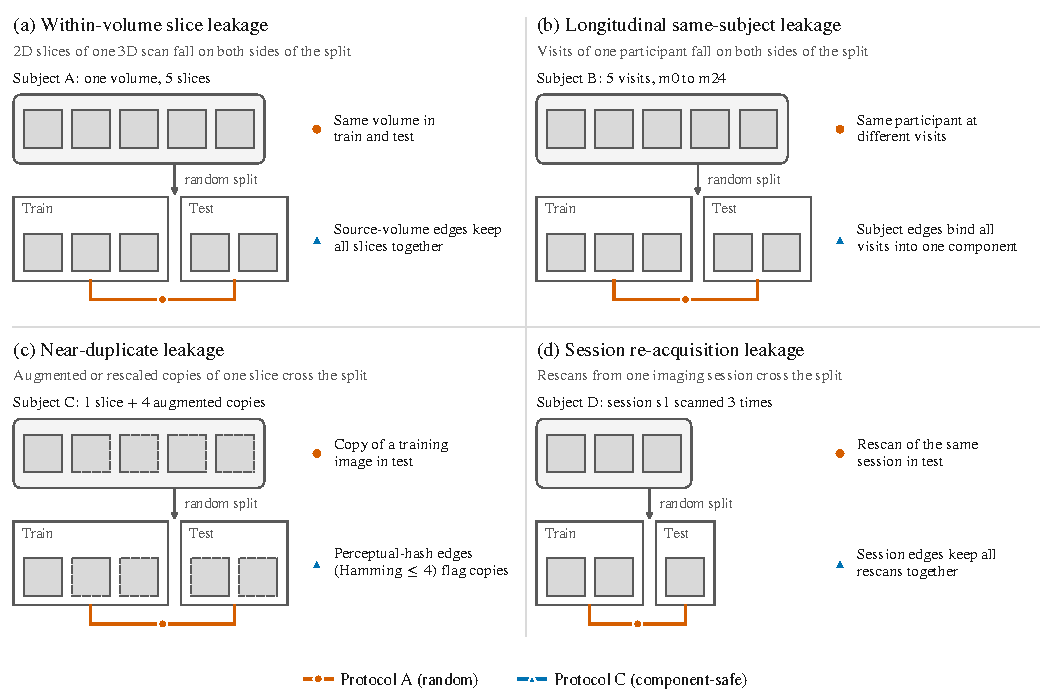
\includegraphics[width=\linewidth]{fig01_leakage_taxonomy.pdf}
\caption{Four leakage modes in slice-based AD MRI benchmarks, and the
\SGA{} edge type that addresses each: (a) source-volume
(series-UID) edges, (b) subject-identifier edges, (c) near-duplicate dHash (Hamming\,$\leq$\,$4$, reported not merged under the default policy), (d) session-identifier edges. In each panel the bracket and circle mark the leak a random split (Protocol~A) produces, and the triangle the edge that prevents it under component-safe splitting (Protocol~C).
Connected components under the union of the blocking edges are the
indivisible split units. \textbf{This figure describes the framework's
design space, not its empirical exercise in this paper.} On the two
source cohorts every connected component contains exactly one
participant; on Tier~1 the components built from the release's own
identifier contain up to three participants each, because that
identifier is not a participant identifier
(\S\ref{sec:data_kaggle}). Modes~(a) and~(d) do fire on ADNI
($209$ source-volume and $223$ session pairs, contributing to $115$ of
the $382$ components), but each joined a pair that mode~(b) had already joined, so no
component differs from a plain subject grouping; mode~(c) is detected
and reported but not merged under the default policy. All four are
implemented and auditable; none is load-bearing on these cohorts,
which is why the component layer's measured marginal over
subject-wise splitting is small
(\S\ref{sec:exp3_degrad}, Supplementary Table~S5). Demonstrating them requires a cohort
with re-acquisition or augmentation structure that subject identity
does not already capture; we name this as the primary
validation gap in \S\ref{sec:limitations}.}
\label{fig:leakage_modes}
\end{figure*}

% ══════════════════════════════════════════════════════════════════════════════
\global\skipbarriertrue
\subsection{The audit instrument}
\label{sec:method}
% ══════════════════════════════════════════════════════════════════════════════

\SGA{} is an open-source reference implementation and audit pipeline, not a general-purpose library: it comprises five sequential
modules (Figure~\ref{fig:pipeline}).

\begin{figure*}[!tb]
\centering
\resizebox{\linewidth}{!}{%
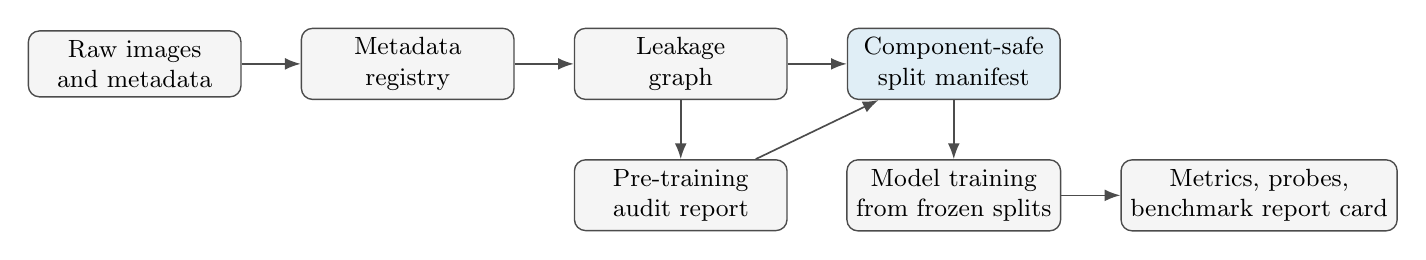
\begin{tikzpicture}[
    node distance=0.75cm,
    box/.style={draw=black!70, line width=0.5pt, rounded corners, align=center,
                minimum width=2.7cm, minimum height=0.8cm, font=\small},
    arrow/.style={-{Latex[length=2mm]}, line width=0.6pt, draw=black!70}
]
\node[box, fill=black!4] (raw) {Raw images\\and metadata};
\node[box, fill=black!4, right=of raw] (registry) {Metadata\\registry};
\node[box, fill=black!4, right=of registry] (graph) {Leakage\\graph};
\node[box, fill=protoC!12, right=of graph] (split) {Component-safe\\split manifest};
\node[box, fill=black!4, below=of graph] (audit) {Pre-training\\audit report};
\node[box, fill=black!4, below=of split] (model) {Model training\\from frozen splits};
\node[box, fill=black!4, right=of model] (report) {Metrics, probes,\\benchmark report card};

\draw[arrow] (raw) -- (registry);
\draw[arrow] (registry) -- (graph);
\draw[arrow] (graph) -- (split);
\draw[arrow] (split) -- (model);
\draw[arrow] (model) -- (report);
\draw[arrow] (graph) -- (audit);
\draw[arrow] (audit) -- (split);
\end{tikzpicture}
}
\caption{The \SGA{} pipeline: from raw images to audit-verified split
         manifests and benchmark report cards.
         Modules are executed sequentially; each produces a versioned
         artefact consumed by the next.}
\label{fig:pipeline}
\end{figure*}

\subsubsection{Metadata registry}
Each image is assigned a row in a manifest with fields including
\texttt{image\_id}, \texttt{subject\_id}, \texttt{subject\_id\_confidence},
\texttt{raw\_class\_label}, \texttt{binary\_label},
\texttt{source\_dataset}, and preprocessing lineage.
For public JPEG benchmarks lacking original DICOM metadata, subject IDs
are inferred from filename conventions with confidence flags for
unparseable cases; Tier~1 shows that such inference can be wrong in
ways no confidence flag detects (\S\ref{sec:data_kaggle}).

\subsubsection{Leakage-graph construction}
\label{sec:leakage_graph}
A leakage graph $G = (V, E)$ is constructed over the image set $V$.
We distinguish the edge families that are \emph{blocking}
(those whose endpoints are merged into one component and therefore can
never be split) from those that are \emph{reported} for inspection, because the
released implementation treats them differently and the distinction
changes what the framework guarantees.

\textbf{Blocking edges.} An edge $(u,v)$ is added, and the endpoints
merged, if $u$ and $v$ share an inferred subject identifier, a session
identifier, a source volume (identified by series UID), an acquisition
date within a subject, or are byte-identical (equal SHA-256). Which of
these are available is cohort-dependent, and the released audit reports
the per-reason edge counts so a reader can see which rules actually
fired: the ADNI tier supplies subject, session, series-UID,
longitudinal and acquisition-date identifiers; the public-benchmark
tier has no acquisition provenance at all, so only inferred subject and
exact-SHA edges exist there. Supplementary Table~S5 gives the
per-cohort breakdown.


The practical consequence is stated plainly: on the two source
cohorts the connected components coincide with participant grouping,
and on Tier~1 they coincide with an identifier that is not
participant identity. The
additional edge families are implemented, auditable and do fire, but
none of them changes a single component here. Establishing their value
requires a cohort whose leakage structure departs from subject identity
(\S\ref{sec:limitations}).

\textbf{Reported edges.} Near-duplicate pairs are detected with a
difference hash (dHash) at $16\times16$, i.e.\ a $256$-bit code, and
flagged when the Hamming distance satisfies $d \leq \delta$ with
$\delta = 4$. Under the default policy
(\texttt{-{}-near-duplicate-policy review}) these pairs are written to a
candidate file and surfaced in the audit report but are \emph{not}
merged; this is the policy under which every manifest and every number
in this paper was produced. A \texttt{blocking} policy that additionally
merges them is implemented and switchable. We keep review as the default
because the identities recovered for Tier~1
(\S\ref{sec:data_kaggle}) let this threshold be calibrated rather
than assumed, and the calibration shows that no setting of it is
safe to gate on. At $d \leq 4$ the detector is precise against
recovered identity (precision $0.986$) but sees only $1.6\%$ of
same-participant pairs, so merging its firings moves the Tier-1 test
contamination from $70.0\%$ to $61.2\%$: real, and nowhere near a
fix. At $d \leq 8$, where it recovers $82\%$ of adjacent-slice
pairs, its $8{,}636$ firings merge the $6{,}400$ images into $27$
components, so the split stops separating anything at all. A further
$1{,}343$ of those firings join images carrying opposite labels and are
refused rather than merged, because the splitter requires label-pure
components: the rule is simultaneously too aggressive to split on and
unable to act on a sixth of what it finds. A rule with that shape
belongs in an audit report a human acts on, not in an automatic gate.

We report the hash family and width explicitly because they are not
interchangeable: dHash at $256$ bits with $\delta=4$ is a far stricter
criterion than the $64$-bit perceptual hashes for which the
$\delta = 4$ convention was originally proposed.
Connected components $C_1, \ldots, C_k$ of $G$ define the atomic units
for splitting: no component may be split across train, validation, and
test partitions.

\subsubsection{Component-safe split generation}
Given target split ratios $r_\text{train} : r_\text{val} : r_\text{test}$
and a class stratification target, \SGA{} assigns entire components to
splits by stratified assignment against image-count targets, seeded for
reproducibility: within each stratum it fills the validation target with
whole components, then the test target from what remains, and leaves the
rest to training. Targets are image counts rather than component counts,
and the test target is the remainder after train and validation are
rounded, so the three never over-subscribe the stratum. On Tier~1 the
subset choice is an exact dynamic-programming solve; on ADNI it is a
greedy descending-size fill approaching the target from below. Ties are
broken on a frozen seeded rank, which is what makes the manifests both
byte-reproducible and genuinely seed-sensitive.
The resulting split manifest is frozen as a CSV file and versioned; no
training script may discover or modify splits at runtime.
Algorithm~\ref{alg:splitguard} formalises the full procedure: leakage
graph construction (lines 1--8) followed by component-safe assignment
(lines 9--18). All randomness is funnelled through the single
\textsc{seed} argument, so the manifest is byte-reproducible.

\begin{algorithm}[!ht]
\caption{\SGA{} leakage-graph construction and component-safe split generation.}
\label{alg:splitguard}
\begin{algorithmic}[1]
\Require image set $V$; subject-ID map $\sigma$; session-ID map
$\varsigma$; source-volume (series-UID) map $\nu$, each defined only where the cohort supplies it;
dHash distance $d(\cdot,\cdot)$ ($256$-bit code) with threshold $\delta = 4$;
near-duplicate policy $\rho \in \{\textsc{review}, \textsc{blocking}\}$
(default \textsc{review}; see \S\ref{sec:leakage_graph});
target ratios $(r_\text{tr}, r_\text{val}, r_\text{te})$;
class label $y : V \to \mathcal{Y}$;
RNG seed $s$
\Ensure split assignment $\pi : V \to \{\text{train}, \text{val}, \text{test}\}$
        such that no leakage component is split across partitions
\State $E \gets \emptyset$;\quad $R \gets \emptyset$
\Comment{$E$: blocking edges; $R$: reported-only pairs}
\For{each pair $(u, v) \in V \times V$ with $u \neq v$}
  \If{$\sigma(u) = \sigma(v)$
       \textbf{ or } $\varsigma(u) = \varsigma(v)$
       \textbf{ or } $\nu(u) = \nu(v)$}
    \State $E \gets E \cup \{(u, v)\}$
    \Comment{subject, session, or source-volume edge, always blocking}
  \ElsIf{$d(u, v) \leq \delta$}
    \If{$\rho = \textsc{blocking}$}
      \State $E \gets E \cup \{(u, v)\}$
    \Else
      \State $R \gets R \cup \{(u, v)\}$
      \Comment{surfaced in the audit report, not merged}
    \EndIf
  \EndIf
\EndFor
\State $\{C_1, \ldots, C_k\} \gets$ connected components of $G = (V, E)$
\State \textit{// Assign whole components, stratified, by image-count targets}
\State $\text{rng} \gets \textsc{RandomGenerator}(s)$
\For{each stratum $S$ (class label; on ADNI also field-strength bucket)}
  \State Freeze a seeded shuffle rank on the components of $S$
  \State $m \gets \sum_{C \in S} |C|$
         \Comment{targets are image counts, not component counts}
  \State $m_\text{tr} \gets \text{round}(r_\text{tr} m)$;\;
         $m_\text{val} \gets \text{round}(r_\text{val} m)$;\;
         $m_\text{te} \gets m - m_\text{tr} - m_\text{val}$
  \State $B_\text{val} \gets \textsc{ChooseSubset}(S, m_\text{val})$
  \State $B_\text{te} \gets \textsc{ChooseSubset}(S \setminus B_\text{val}, m_\text{te})$
  \State $B_\text{tr} \gets S \setminus (B_\text{val} \cup B_\text{te})$
         \Comment{remainder; never chosen explicitly}
\EndFor
\Statex \textit{// \textsc{ChooseSubset}$(S,m)$: on ADNI, visit $S$ by $|C|$
         descending with ties broken on the frozen rank and take each
         component that still fits in the remaining budget, approaching $m$
         from below; on Tier~1, solve the same objective exactly by
         dynamic programming over attainable sums.}
\State $\pi \gets$ assignment induced by $(B_\text{tr}, B_\text{val}, B_\text{te})$
\State \textbf{return} $\pi$, audit report $\{$component sizes, class balance,
        cross-partition contamination, source/site/demographic associations$\}$
\end{algorithmic}
\end{algorithm}

\paragraph{Implementation note}
The double loop on lines 2--6 of Algorithm~\ref{alg:splitguard} is
shown in $\mathcal{O}(N^2)$ form for clarity; in implementation,
exact identifier edges (subject, session, series UID, acquisition date,
SHA-256) use hash-grouping in $\mathcal{O}(N)$. The near-duplicate
comparison is the exception: it is currently evaluated over all
$\binom{N}{2}$ pairs, which is tractable at the scale studied here
($N \leq 6{,}400$) but is the component that would need
locality-sensitive indexing before the framework is applied to
repositories of $10^5$ images or more. Identifier-edge construction
completes in $<1$~ms per cohort on a consumer CPU, so framework
runtime is dominated by image ingestion and by the pairwise hash
comparison.

\paragraph{Protocol nomenclature}
Throughout the experiments we evaluate three split protocols on the
same image universe:
\begin{description}
  \item[Protocol A (Random, leaky).] Random image-level shuffle into
        train/val/test; the conventional benchmark setup.
  \item[Protocol B (Subject-only).] Split by inferred subject identity:
        all images from one subject land in a single partition, but
        connected-component and near-duplicate safety are \emph{not}
        enforced. When subject identity is unavailable, or when leakage
        components coincide with subject boundaries, Protocol~B is not
        separately informative from Protocol~C; we therefore report it
        only where it isolates a distinct safety layer (the ADNI
        experiments in \S\ref{sec:exp6_adni}).
  \item[Protocol C (Component-safe, \SGA{}).] Full leakage-graph
        component-safe split: subject identity, scanner-session
        re-acquisitions, and near-duplicate components are all
        respected.
\end{description}
The three protocols form a strict ordering (A $\supseteq$ B $\supseteq$ C)
in terms of leakage permissiveness; the three-point degradation analysis
in \S\ref{sec:exp3_degrad} traces the contribution of each layer.

\subsubsection{Pre-training audit}
Before training, \SGA{} emits a structured audit report with three parts:
(i) component overlap across partitions; (ii) label distribution per
partition; and (iii) association between label and each audited covariate,
given as Cram\'{e}r's $V$ per partition. The covariates are site code
(extracted from the ADNI \texttt{PTID}), scanner field strength and sex.

This last part is complementary to scanner-effect work~\cite{glocker2019scanner}
and to harmonisation in the ComBat
lineage~\cite{johnson2007combat,fortin2017combat,pomponio2020lifespan}.
\SGA{} surfaces such confounds but does not remove them, because the gap
measured here is dominated by the subject-identity channel, which
post-hoc harmonisation does not address. The clinical claim-boundary
statement in the report card (\S\ref{sec:discussion}) is authored, not
emitted by the audit.
The audit report issues a binary GO / NO-GO decision for training
according to the formal criteria in Supplementary Table~S6.


\subsubsection{Model audit layer}
\label{sec:model_audit}
After training, \SGA{} evaluates trained model representations with a
linear probe: probe accuracy above chance indicates residual shortcut
encoding. In this release only the \emph{subject-identity} probe is
implemented and reported (\S\ref{sec:exp2_probe},
\texttt{scripts/\pb run\_biometric\_probe\_adni.py}), because
subject identity is the channel the component-safe split is designed
to close. Probes for dataset source, site/scanner, and demographic
attributes follow the same construction and are the natural extension
of this layer, but are not implemented in v1 and no such probe result
is reported here; the site--label association we do report
(\S\ref{sec:exp6_adni}) is a metadata-level contingency statistic, not
a representation-level probe.

% ══════════════════════════════════════════════════════════════════════════════
\subsection{Cohorts}
\label{sec:data}
% ══════════════════════════════════════════════════════════════════════════════

\paragraph{Cohort roles}
Two source cohorts carry the measurements. The
\textbf{ADNI1: Complete 3Yr 1.5T} collection (\S\ref{sec:data_adni})
is the paper's \emph{headline} cohort: all headline numerical claims
in the abstract, the cost-of-leakage analysis, the subgroup analysis,
and the dose-response stress test derive from it.
\textbf{OASIS-1} (\S\ref{sec:data_oasis}) is the replication cohort, where
participant identifiers are authoritative. It is operationally external to
ADNI: a different recruiting site, scanners, acquisition protocols and
recruitment era. The direction-preservation we report between the two
cohorts is therefore a partial cross-site generalisation check, not
external validation in the regulatory sense. The third tier is not a third cohort. The \textbf{Kaggle
public JPEG benchmark} (\S\ref{sec:data_kaggle}) is, as we show by
content matching, a redistribution of OASIS-1 itself whose
participant identifiers have been replaced by a filename index that
both merges and splits participants. We therefore use it for what it
documents rather than for what it would replicate: an observed and
measurable instance of the provenance damage that
\S\ref{sec:provenance_degradation} otherwise has to simulate.
Throughout the experiments we use the shorthand \emph{Tier~1}
(redistributed public benchmark), \emph{Tier~2} (OASIS-1),
\emph{Tier~3} (ADNI1 headline) for brevity.

\subsubsection{Tier 1: a redistributed public benchmark}
\label{sec:data_kaggle}
The widely distributed public Kaggle Alzheimer's MRI benchmark
dataset~\cite{kaggle_ad_4class} comprises $6{,}400$ JPEG images of
uniform $176 \times 208$ pixels in four severity classes:
NonDemented ($n = 3{,}200$), VeryMildDemented ($n = 2{,}240$),
MildDemented ($n = 896$), and ModerateDemented ($n = 64$). The
release states no origin, carries no acquisition metadata, and
exposes subject identity only through a parenthesised filename index
(\eg{} \texttt{NonDemented\_patient100\_1 (100).jpg}).

\paragraph{What the images are}
We recovered the origin by content. Every image was matched against
axial slices of all $436$ OASIS-1 cross-sectional volumes in their
processed, atlas-registered, masked form
(\texttt{T88\_111/*\_masked\_gfc};
\texttt{scripts/\pb audit\_tier1\_ground\_truth.py}). All $6{,}400$
images match unambiguously: the lowest correlation between an image
and its matched slice is $0.9996$, while the highest correlation any
image reaches with a slice of a \emph{different} participant is
$0.9623$. The benchmark is $200$ OASIS-1 participants at $32$
consecutive axial slices each (atlas slices $71$--$102$). The folder labels
reproduce those participants' Clinical Dementia Rating exactly, for
every one of the $6{,}400$ images ($\text{CDR} = 0 \rightarrow$
NonDemented, $0.5 \rightarrow$ VeryMild, $1 \rightarrow$ Mild,
$2 \rightarrow$ Moderate), and no participant's slices are split
across two folders: they are CDR, not the weak folder-derived labels
they are usually assumed to be. Every one of the $200$
participants is also in our Tier-2 OASIS-1 set, so Tier~1 and Tier~2
are two views of one cohort, and the cross-tier replication in this
paper rests on two source cohorts rather than three.

\paragraph{What redistribution destroyed}
The filename index is not a participant identifier. Its $324$
distinct keys divide into $149$ that correspond to exactly one
participant and $175$ that merge two or three participants under a
single key, while $179$ of the $200$ participants are spread across
two or more keys and one is spread across $32$. A further $128$
images ($2.0\%$) carry no parsable index at all. Grouping by this key
is therefore not subject-wise splitting: it is grouping on a key that
is wrong in both directions at once, and the supplied identifier alone
does not reveal that. Recovering it required matching the images against
the source cohort, which a user of the release is not placed to do.

Against the recovered identities the damage is exact. In the frozen
seed-42 split used throughout this paper, which groups by the
filename key, $85$ participants have images in more than one
partition, $46$ of the $58$ test participants also appear in
training, and $647$ of the $960$ test images ($67.4\%$) belong to a
participant the model was trained on. Table~\ref{tab:tier1_rules}
repeats that measurement for every grouping rule the release
supports.

\begin{table*}[!tb]
\centering
\footnotesize
\caption{Every grouping rule the Tier-1 release supports, measured
against the recovered participant identities over five seeds.
Contamination is the share of test images whose participant also
appears in training. The filename key, the only identifier the
release provides, leaves seven test images in ten contaminated.
Near-duplicate edges at $d \leq 4$ remove an eighth of that; at
$d \leq 8$ the graph collapses ($8{,}636$ pairs merge the corpus into
$27$ components, the largest holding $3{,}117$ images, while a further
$1{,}343$ firings join opposite-label images and are refused rather than
merged), which is a different failure rather than a fix. Only the recovered participant
identity yields a clean split.}
\label{tab:tier1_rules}
\begin{tabular}{@{}lrrlr@{}}
\toprule
Grouping rule & Components & Largest & Test contamination & Test participants \\
              &            & (images) & mean [min, max] & in train / total \\
\midrule
Filename key (release identifier)   & 324 & 32      & $70.0\%$ $[62.0, 78.6]$ & $46.4 / 59.4$ \\
\quad $+$ near-duplicate $d \leq 4$ & 219 & 192     & $61.2\%$ $[53.4, 67.5]$ & $42.0 / 56.2$ \\
\quad $+$ near-duplicate $d \leq 8$ & 27  & 3{,}117 & $100\%$                 & $1.0 / 1.0$ \\
Near-duplicate $d \leq 8$ alone     & 999 & 1{,}770 & $99.5\%$ $[99.0, 100]$  & $104.4 / 105.0$ \\
Recovered participant               & 200 & 32      & $0\%$                   & $0 / 29.0$ \\
\bottomrule
\end{tabular}
\end{table*}

\paragraph{Near-duplicate structure, read against ground truth}
No exact SHA-256 duplicates exist. The near-duplicate detector (dHash
at $16 \times 16$, a $256$-bit code, Hamming $d \leq 4$) flags
$1{,}582$ candidate pairs, of which $1{,}559$ ($98.5\%$) join two
slices of the same participant and $1{,}526$ join slices one position
apart in the same volume. Of the $57$ pairs that straddle the frozen
partitions, the recovered identities make $52$ the same participant
and $5$ different participants. The filename key had called $36$ of
those $57$ pairs ``different subjects''; in $31$ of them the key was
wrong and the detector was right. Read against the release's own
identifier the detector looks like a $63\%$ false-positive rate; read
against ground truth its cross-partition output is $91\%$ true
leakage. Only the recovered provenance distinguishes the two
readings, which is the point: an audit that can only compare a
detector against the identifiers it already has will systematically
mistake a broken identifier for a false alarm.

\paragraph{Calibrating the detector}
With every pair's identity known, the threshold can be calibrated
over all $20{,}476{,}800$ pairs instead of argued for. At $d \leq 4$
the detector is precise and sparse: precision $0.986$ and recall $0.246$ of
adjacent-slice pairs, which is $0.016$ of all pairs sharing a
participant, at a false-positive rate of $1.1 \times 10^{-6}$. At $d \leq 8$ it is
sensitive and unusable as a blocking rule: precision $0.699$, recall
$0.816$ of adjacent slices, false-positive rate
$1.3 \times 10^{-4}$, which at this corpus size is the $8{,}636$
pairs that collapse the graph in Table~\ref{tab:tier1_rules}. The
median Hamming distance between two slices of the same participant is
$33$ bits against $35$ between participants, so what the detector
separates is \emph{neighbouring slices}, not participants. This is
the precise sense in which perceptual hashing cannot stand in for a
participant identifier.

\subsubsection{Tier 2: OASIS-1}
\label{sec:data_oasis}
We use OASIS-1 as the metadata-rich replication
cohort~\cite{oasis1}; LaMontagne \etal~\cite{lamontagne2019oasis3}
describe the successor OASIS-3 longitudinal release for context.
All 12 official raw cross-sectional archives were available locally,
together with the demographic/clinical and reliability spreadsheets.
The clinical spreadsheet contains 436 session rows from 416 unique
subjects, including 20 MR2 reliability sessions.
For each session, \SGA{} selectively extracts one processed masked T88
MPRAGE Analyze pair
(\texttt{PROCESSED/\pb MPRAGE/\pb T88\_111/\pb *\_masked\_gfc.img/\pb .hdr}) without
fully expanding the raw archives.

CDR is used as the primary clinical label: CDR \(=0\) is mapped to
NonDemented, and CDR \(>0\) to Demented.
Sessions with missing CDR are retained in the manifest for auditability
but excluded from the primary classification experiment.
The resulting OASIS-1 manifest contains 135 NonDemented sessions,
100 Demented sessions, and 201 sessions with missing CDR.
Five central coronal slices are derived from each processed volume,
yielding 2,180 total slices and 1,175 labelled slices
(675 NonDemented, 500 Demented).
The frozen OASIS-1 \SGA{} split contains 825/175/175 labelled slices in
train/validation/test, with 165/35/35 subjects respectively and zero
subject or component overlap across splits.

\subsubsection{Tier 3: ADNI1 Complete 3Yr 1.5T (headline cohort)}
\label{sec:data_adni}
We use the ADNI1: Complete 3Yr 1.5T image collection as the paper's
headline cohort, accessed under an active LONI IDA Data Use Agreement;
the consortium overview~\cite{adni}, the MRI-acquisition
protocol~\cite{jack2008adnimri}, and the clinical-characterisation
core~\cite{petersen2010adniclinical} provide the foundational
methodology references for the ADNI release used here. All headline
numerical claims in the abstract, the intro, and the cost-of-leakage
and dose-response analyses derive from this cohort.
The collection contains 2,182 pre-processed 1.5T T1-weighted volumes
(MPR or MPR-R variants with GradWarp, B1 correction, N3, and intensity
scaling already applied) from 382 unique subjects spanning the
ADNI1/GO/2/3/4 phases (Table~\ref{tab:adni_demographics}).
A small subset (28 scans, 17 of which fall in the CN/AD universe) are
magnetization-transfer T1 (MT1) acquisitions rather than MPRAGE; these
are retained in the primary analysis and excluded in a pre-specified
sensitivity arm (\S\ref{sec:exp6_adni}).

% Auto-generated by scripts/generate_adni_paper_tables.py.
% Do not hand-edit; regenerate from the manifest + PTDEMOG + MMSE.
\begin{table}[!tb]
\centering
\caption{ADNI1: Complete 3Yr 1.5T cohort demographics. Subject-level summary; subjects are assigned to a diagnosis group by highest-priority label observed across all visits (AD $>$ CN $>$ MCI). Age computed at each subject's earliest scan from \texttt{PTDOBYY}; baseline MMSE is each subject's earliest non-missing \texttt{MMSCORE}.}
\label{tab:adni_demographics}
\begin{tabular}{lrrrr}
  \toprule
  & \textbf{CN} & \textbf{MCI} & \textbf{AD} & \textbf{Total} \\
  \midrule
  Subjects ($n$) & 142 & 68 & 172 & 382 \\
  Scans ($n$) & 794 & 442 & 946 & 2182 \\
  Age, years (mean $\pm$ SD) & 75.7 $\pm$ 5.4 & 75.1 $\pm$ 7.1 & 75.0 $\pm$ 7.3 & n/a \\
  Female ($n$, \%) & 68 (48\%) & 15 (22\%) & 76 (44\%) & n/a \\
  Baseline MMSE (mean $\pm$ SD) & 29.2 $\pm$ 1.0 & 27.5 $\pm$ 1.7 & 24.7 $\pm$ 2.5 & n/a \\
  \bottomrule
\end{tabular}
\end{table}


\begin{figure*}[!tb]
\centering
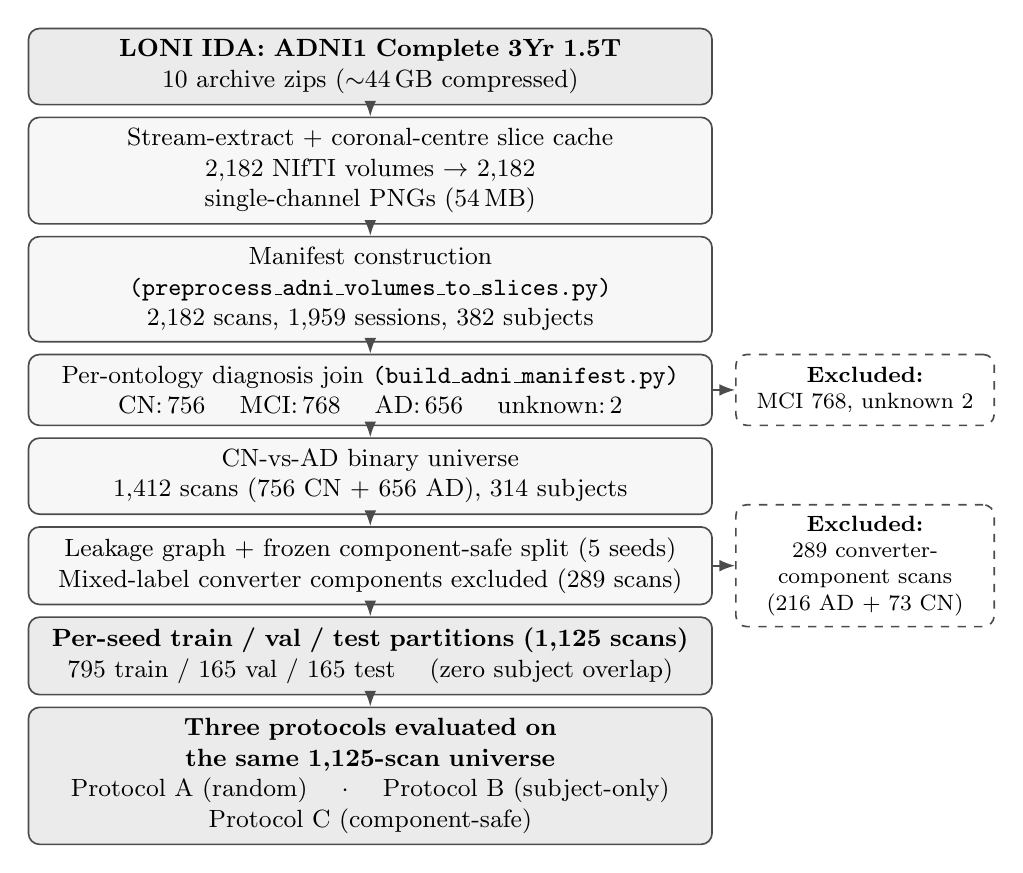
\begin{tikzpicture}[
    node distance=4pt,
    every node/.style={font=\small},
    main/.style={draw=black!70, rounded corners, fill=black!8, align=center,
                 inner sep=4pt, text width=8.4cm, minimum height=0.9cm,
                 line width=0.6pt},
    derived/.style={draw=black!70, rounded corners, fill=black!3, align=center,
                    inner sep=4pt, text width=8.4cm, minimum height=0.9cm,
                    line width=0.6pt},
    audit/.style={draw=black!70, dashed, rounded corners, fill=white, align=center,
                  inner sep=4pt, text width=3.0cm, minimum height=0.9cm,
                  line width=0.6pt, font=\footnotesize},
    arrow/.style={-{Latex[length=2.0mm]}, line width=0.6pt, draw=black!70},
]
% Main column boxes (top to bottom)
\node[main]    (loni)    {\textbf{LONI IDA: ADNI1 Complete 3Yr 1.5T}\\
                          10 archive zips ($\sim$44\,GB compressed)};
\node[derived] (extract) [below=of loni]    {Stream-extract + coronal-centre slice cache\\
                                              2,182 NIfTI volumes $\rightarrow$ 2,182 single-channel PNGs (54\,MB)};
\node[derived] (manifest) [below=of extract] {Manifest construction \texttt{(preprocess\_adni\_volumes\_to\_slices.py)}\\
                                              2,182 scans, 1,959 sessions, 382 subjects};
\node[derived] (diag)     [below=of manifest] {Per-ontology diagnosis join \texttt{(build\_adni\_manifest.py)}\\
                                               CN:\,756 \quad MCI:\,768 \quad AD:\,656 \quad unknown:\,2};
\node[derived] (cnad)     [below=of diag]     {CN-vs-AD binary universe\\
                                               1,412 scans (756 CN + 656 AD), 314 subjects};
\node[derived] (leakgraph) [below=of cnad]    {Leakage graph + frozen component-safe split (5 seeds)\\
                                               Mixed-label converter components excluded (289 scans)};
\node[main]    (split)     [below=of leakgraph] {\textbf{Per-seed train / val / test partitions (1,125 scans)}\\
                                                  795 train / 165 val / 165 test \quad (zero subject overlap)};
\node[main]    (protocols) [below=of split]    {\textbf{Three protocols evaluated on the same 1,125-scan universe}\\
                                                 \mbox{Protocol~A (random)} \quad $\cdot$ \quad \mbox{Protocol~B (subject-only)}\\
                                                 \mbox{Protocol~C (component-safe)}};

% Right-side exclusion boxes
\node[audit] (mciex)    [right=8pt of diag]      {\textbf{Excluded:}\\ MCI 768, unknown 2};
\node[audit] (orphanex) [right=8pt of leakgraph] {\textbf{Excluded:}\\ 289 converter-component scans\\(216 AD + 73 CN)};

% Vertical arrows down the main column
\draw[arrow] (loni)      -- (extract);
\draw[arrow] (extract)   -- (manifest);
\draw[arrow] (manifest)  -- (diag);
\draw[arrow] (diag)      -- (cnad);
\draw[arrow] (cnad)      -- (leakgraph);
\draw[arrow] (leakgraph) -- (split);
\draw[arrow] (split)     -- (protocols);

% Right-side exclusion arrows
\draw[arrow] (diag.east)      -- (mciex.west);
\draw[arrow] (leakgraph.east) -- (orphanex.west);
\end{tikzpicture}
\caption{ADNI1: Complete 3Yr 1.5T data flow from LONI IDA archive
download to per-seed train/validation/test partitions. Each transition
annotates the row count and the script responsible
(\texttt{preprocess\_adni\_volumes\_to\_slices.py},
\texttt{build\_adni\_manifest.py},
\texttt{make\_adni\_splitguard\_split.py}).
Dashed boxes on the right record exclusions: MCI / unknown diagnoses excluded
from the CN-vs-AD task by construction, and 289 CN/AD scans
(216 AD + 73 CN) from mixed-label longitudinal converter components
excluded from the primary arm and re-included in the sensitivity arm
(\S\ref{sec:exp6_adni}).}
\label{fig:adni_dataflow}
\end{figure*}

Diagnosis labels are taken from the ADNI diagnostic summary table
(\texttt{DXSUM\_PDXCONV\_ADNIALL}) under a phase-aware visit-level
mapping. Every visit in the export we use carries the canonical
\texttt{DIAGNOSIS} code (1=CN, 2=MCI, 3=AD), and all $2{,}180$ resolved
labels in the released manifest come from it
(\texttt{label\_source=DIAGNOSIS}). The released builder also
implements two fallbacks for exports that differ from ours: a
longitudinal \texttt{DXCHANGE} collapse to the destination state, and
the mutually exclusive ADNI1 legacy flags \texttt{DXAD},
\texttt{DXMCI}, \texttt{DXNORM}, which some ADNI1 case report forms
use instead of one categorical field. Neither fallback fires on this
export, which has no \texttt{DXCHANGE} column at all, so neither
contributes a label reported here; we describe them because they are in
the released code, not because they shaped these results. Scan-to-visit alignment uses a 180-day date-proximity join
through the MRI metadata table, with a documented date-only fallback
when the viscode-keyed lookup fails. The full mapping rule and edge-case
handling are pre-specified before any model training; the resulting
manifest yields 756 CN, 768 MCI, and 656 AD scans, plus two scans whose
diagnosis cannot be resolved (kept in the manifest with
\texttt{diagnosis\_group=unknown} for auditability and excluded from
the primary CN-vs-AD task).

\paragraph{Linkage-integrity audit}
Because every ADNI label in this study rests on this join, we
account for it per scan in \texttt{adni\_linkage\_audit.csv}
(\texttt{scripts/\pb build\_linkage\_audit.py}; schema in Supplementary
Material~S5). The table is an ADNI-derived Tier-3 artefact and is
therefore not redistributed with the release; the LONI data-use
agreement permits only hashed derivatives, which a reader with ADNI
access regenerates from their own download by running that script. Each row records the scan identifier, a salted PBKDF2
derivation of the participant identifier, the acquisition date, the
join tier, the source column, and whether the scan enters the CN-vs-AD
universe. Of the $2{,}182$ scans, $1{,}695$ ($77.7\%$) were labelled
through a direct \texttt{(RID, VISCODE)} match, $485$ ($22.2\%$)
required the 180-day date-proximity fallback, and $2$ ($0.1\%$)
remained unresolved; these last two are the
\texttt{diagnosis\_group=unknown} scans discussed above. That roughly
one label in five depends on a date match rather than an exact visit
key is a real limitation of the label chain, and stating it is not
enough: we also measure what it costs. The primary arm is the worst
case for it. Of its $1{,}123$ CN-vs-AD scans, $841$ are labelled through the exact
visit key and $282$ ($25.1\%$) through the date fallback. That share
exceeds the whole CN-vs-AD universe's $297$ of $1{,}412$ ($21.0\%$, against
$1{,}115$ on the exact key), because the converter components this arm
excludes are almost fully covered by the visit key ($5.2\%$ date-only). The
exact-linkage arm of \S\ref{sec:exp6_adni} therefore retrains all
three protocols on the $841$, keeping the same $220$ participants, and
asks whether the headline gap rests on the weaker quarter of the label
chain. Participant identifiers are hashed under a
secret per-release salt for the same reason as the Tier-3 manifest:
ADNI PTIDs are low-entropy, so a published salt would make the file
re-identifiable.

For apples-to-apples comparison with Tier 2, each volume is reduced to
a single 2D coronal-centre slice. The slice is computed once at ingest
with 1st--99th percentile intensity normalisation and saved as a
single-channel PNG; this caching step is byte-identical to the
volume-time computation in \S\ref{sec:data_oasis} but fits the full
collection in 54\,MB rather than 77\,GB of NIfTI volumes. The leakage
graph links scans sharing a subject identifier, a session identifier, a
series UID, or an acquisition date; these four rules fire on $1{,}800$,
$223$, $209$ and $222$ pairs respectively. The ADNI builder computes no
image-hash edges, by design and not by omission, so this tier carries no
near-duplicate protection: that channel is measured on Tier~1, where the
images are public and may be hashed and redistributed. The 382-subject
collection collapses into 382 single-subject components (mean 5.7 scans
per component, range 4--11), so the frozen \SGA{} split is effectively a
subject-stratified partition with additional session-, series- and
date-level edges that, on this cohort, every one of which is subsumed by
the subject rule (\S\ref{sec:provenance_degradation}).

The CN-vs-AD binary task universe excludes 768 MCI scans by
construction (the binary task is cross-sectional, not longitudinal
progression-prediction) and a further $289$ scans
($216$ AD + $73$ CN) drawn from components tagged
\texttt{mixed\_\allowbreak{}label}: subjects whose visit
sequence crosses CN, MCI, and AD diagnoses (longitudinal converters).
Including those subjects in the primary arm would require either
(i) breaking the subject-level partition (the same subject
contributes CN visits to one split and AD visits to another), or
(ii) collapsing their longitudinal trajectory to a single subject-level
label, which conflates cross-sectional CN-vs-AD classification with
progression-prediction. We adopt the cleaner option: exclude these
$289$ scans from the primary arm and re-include them in a
pre-specified sensitivity arm (\S\ref{sec:exp6_adni},
``Sensitivity to converter exclusion''), assigning each mixed-label
component a CN-or-AD majority label for stratification only. No scan is
relabelled: training and evaluation use each scan's own visit-level
diagnosis throughout, so a converting participant contributes CN scans
as CN and AD scans as AD within one component. The total inflation
gap in the sensitivity arm (\AdniConvGap{}) is \emph{larger} than in
the primary arm (\AdniGapTotal{}), so the exclusion does not drive the
headline result.
Removing these $289$ scans leaves $1{,}123$ CN/AD scans. The frozen
split manifests carry $1{,}125$ rows, because two scans whose
visit-level diagnosis did not resolve
(\texttt{diagnosis\_group=unknown}, \S\ref{sec:data_adni}) are kept in
the manifest and flagged there rather than deleted from it. They are
not, however, evaluated: every trainer maps only CN and AD to a target
and silently skips any other value, so the two rows enter no partition
the model sees. The evaluated universe is therefore $1{,}123$ scans
across 220 single-subject components, equivalently 220 participants,
since every component here contains exactly one subject. Under
component-safe splitting each frozen seed produces train/validation/test
partitions of $793/165/165$ evaluated scans; the manifest row counts are
two higher. We record the discrepancy rather than reconciling it
silently, because a manifest row count and an evaluated scan count are
different quantities and conflating them is how a cohort size drifts. Figure~\ref{fig:adni_dataflow} summarises the
end-to-end pipeline from the 10 LONI IDA archive zips through the
slice-cached manifest to the per-seed splits.

% ══════════════════════════════════════════════════════════════════════════════
\section{Results}
\label{sec:experiments}
% ══════════════════════════════════════════════════════════════════════════════

\paragraph{Statistical conventions}
Unless stated otherwise, intervals are $B = 10{,}000$ paired-seed
bootstrap intervals~\cite{efron1986bootstrap,carpenter2000bootstrap}
over a five-seed array. At $n = 5$ they describe seed-level variability
rather than population-level uncertainty, and the ``$95\%$'' label is
kept only for tabulation convention. Where we say a direction holds,
we mean the sign of the inter-protocol delta is the same in every one
of the five seeds; we do not quote the resample count, because
resampling five same-signed numbers reproduces that sign with
probability one and so adds nothing to the seed count itself. A
two-level hierarchical (subject\,$\times$\,seed) bootstrap is run on
every arm from its per-image predictions and reported alongside; it is
the more defensible inferential quantity and is roughly
$1.9$--$4.7\times$ wider across the arms. We weight, in decreasing order, effect size,
sign consistency, the hierarchical interval, and last the paired-seed
width.

\paragraph{Training recipe and compute}
The three 2D cohorts and both 2D backbones share one recipe:
ImageNet-pretrained ResNet-18 (or DenseNet-121 in the architecture arms),
$3\!\times\!224\!\times\!224$ input with ImageNet mean/std
normalisation, horizontal flip and $\pm 7^{\circ}$ rotation
augmentation, AdamW with cosine annealing, weight decay $10^{-2}$,
class-weighted BCE loss and one-shot test-set evaluation.
Cohort-specific settings are learning rate $3\!\times\!10^{-4}$
(Tier~1, OASIS-1) or $10^{-4}$ (ADNI); $30$, $20$ and $15$ epochs;
batch size $32$ on Tier~1 and OASIS-1 and $16$ on ADNI; seeds
$\{42,0,1,2,3\}$ on Tier~1 and OASIS-1 and $\{0,1,2,3,4\}$ on ADNI.
The volumetric arm departs from that recipe in three ways that matter
for reading it: a 3D ResNet-18 on $128^3$ volumes at batch size $4$ for
$15$ epochs, trained from random initialisation rather than ImageNet
weights, on z-scored volumes with no augmentation. Tier~1 additionally
trains under CUDA mixed precision, which the other arms do not use. An early
version of the volumetric trainer computed $1-\mathrm{AUROC}$ from a
descending rank sum, which would have selected the least-trained epoch of every
run; it was corrected before this arm was trained, and the released code carries
a regression test for it. Every run was executed in one code state with
deterministic cuDNN kernels and seeded data loaders, on one NVIDIA H100
except the dose-response matrix, rerun on an NVIDIA RTX PRO 4500, the
volumetric arm, run on an NVIDIA RTX 2000 Ada, and the exact-linkage,
structured-corruption and label-permutation arms, run on an NVIDIA RTX
4090 (\S Declarations);
the full configuration is in Supplementary Table~S1.

\subsection{Observed provenance damage on a redistributed benchmark}
\label{sec:exp1}

\paragraph{Setup}
Tier~1 is trained under three protocols that differ only in what they
group by. Protocol~A shuffles images at random. Protocol~B$'$ groups by
the filename key, the only identifier the release carries and therefore
the strongest protocol an audit run from inside the release can
implement. Protocol~C$'$ groups by the participant identity recovered in
\S\ref{sec:data_kaggle}. Everything else is held fixed. The backbone is
ResNet-18~\cite{he2016} with ImageNet pre-trained weights, trained for $30$
epochs at batch size $32$ with random horizontal flip and $\pm 7^\circ$
rotation. The optimiser is AdamW ($\beta_1 = 0.9$, $\beta_2 = 0.999$,
$\epsilon = 10^{-8}$, AMSGrad disabled) at learning rate
$3 \times 10^{-4}$ and weight decay $10^{-2}$, with cosine annealing and a
class-frequency-weighted BCE loss. The seed array is $\{42, 0, 1, 2, 3\}$.

\paragraph{Leakage verification}
Under Protocol~A, $195$ of $219$ test-set filename keys ($89.0\%$) also
appear in training. Under Protocol~B$'$ no filename key crosses a
partition, so an audit restricted to the release's own metadata reports
zero leakage, while $70.0\%$ of the test images in fact belong to a
participant the model trained on. Under Protocol~C$'$ the contamination
is zero (Table~\ref{tab:tier1_rules}).

\paragraph{Results}
% Generated by scripts/gpu_postprocess.py. Do not edit by hand.
\begin{table*}[!tb]
\centering
\caption{Tier-1 test AUROC under the three grouping rules, five seeds. Protocol~B$'$ groups by the filename key the release ships, which is the best an audit inside the release can do; Protocol~C$'$ groups by the participant identity recovered from OASIS-1. The gap column is A$-$C$'$.}
\label{tab:tier1_truth}
\footnotesize
\begin{tabular}{lrrrr}
\toprule
\textbf{Seed} & \textbf{A: random} & \textbf{B$'$: filename key} & \textbf{C$'$: participant} & \textbf{Gap (A$-$C$'$)} \\
\midrule
42 & 0.9994 & 0.8581 & 0.8387 & \gap{+0.161} \\
0 & 0.9999 & 0.7508 & 0.7655 & \gap{+0.234} \\
1 & 0.9996 & 0.8142 & 0.7496 & \gap{+0.250} \\
2 & 0.9976 & 0.7834 & 0.7743 & \gap{+0.223} \\
3 & 0.9999 & 0.7574 & 0.7030 & \gap{+0.297} \\
\midrule
\textbf{Mean $\pm$ SD} & $0.999 \pm 0.001$ & $0.793 \pm 0.044$ & $0.766 \pm 0.049$ & \gap{+0.233} \\
\bottomrule
\end{tabular}
\end{table*}


Random splitting inflates test AUROC from \TierOneTrueAUROC{} to
\TierOneRandomAUROC{}, a gap of \TierOneGapTotal{}. That part is the
familiar result. The part this tier exists for is the middle column:
grouping by the release's own identifier recovers
\TierOneShareFilename\% of that gap and leaves \TierOneGapResidual{}
AUROC of inflation standing, because the key it groups on merges and
splits participants. A practitioner who does everything correctly with
the information the benchmark provides still reports an inflated number,
and nothing inside the benchmark reveals it. This is the difference
between leakage as a protocol error, which the literature already
documents, and leakage as a provenance failure, which survives a
correctly applied protocol.
Figure~\ref{fig:tier1_overview} separates what is stable across seeds
from what is not. Protocol~A sits above both grouped protocols in all
five seeds (Figure~\ref{fig:seed_stability}) and on every metric at
seed $=42$ (Figure~\ref{fig:metrics}), so the headline gap is not a
seed artefact. The residual between B$'$ and C$'$ is the smaller
quantity and it is not uniform: their AUROC ordering reverses in one
seed of five (Table~\ref{tab:tier1_truth}), and at seed $=42$ C$'$ is
the more specific of the two while B$'$ is the more sensitive, which is
what a threshold applied to a less separable score produces. The
\TierOneGapResidual{} residual is therefore a five-seed mean and not a
per-run guarantee, and we hold it to the same standard as the ADNI
component marginal rather than a softer one: its
subject\,$\times$\,seed interval is $[-0.058, +0.113]$, which spans
zero, exactly as ADNI's \AdniMarginal{} \AdniMarginalCI{} does. Both
are unresolved at five seeds and we report both that way. What the
Tier-1 tier establishes is therefore the \emph{contamination}, which is
structural and needs no interval -- $70\%$ of test images share a
participant with training under the release's own key -- not the AUROC
consequence of that contamination, which these five seeds cannot pin
down. The distinction matters because the contamination is what a
practitioner can check and the AUROC consequence is what they would
have to take on faith.

\begin{figure*}[!tb]
\centering
\begin{subfigure}[t]{0.85\linewidth}
  \centering
  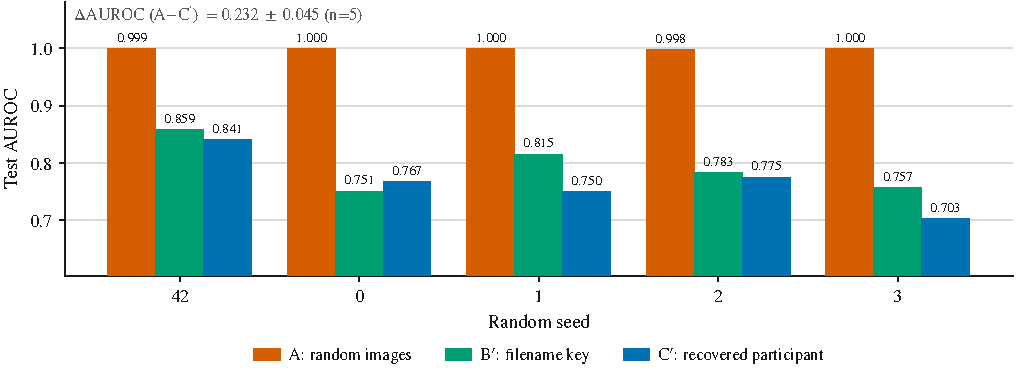
\includegraphics[width=\linewidth]{fig04a_seed_stability.pdf}
  \caption{Per-seed test AUROC under the three grouping rules.}
  \label{fig:seed_stability}
\end{subfigure}\\[0.2em]
\begin{subfigure}[t]{0.85\linewidth}
  \centering
  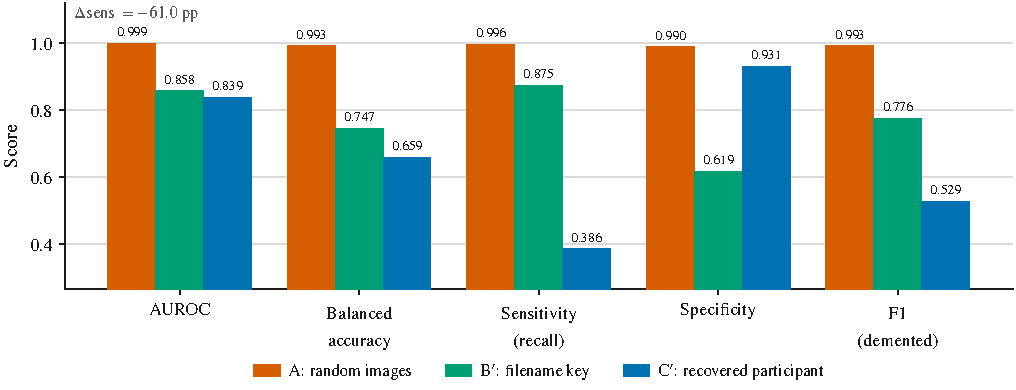
\includegraphics[width=\linewidth]{fig04b_metric_comparison.pdf}
  \caption{All test-set metrics at seed $= 42$.}
  \label{fig:metrics}
\end{subfigure}
\caption{Tier-1 under random splitting (A, vermilion), the release's
         filename key (B$'$, green) and recovered participant identity
         (C$'$, blue): (a) seed stability, and (b) the per-metric
         breakdown. Panels are stacked vertically rather than
         side-by-side so that the in-figure tick labels and bar
         annotations remain legible at print size.}
\label{fig:tier1_overview}
\end{figure*}

\paragraph{What the three test sets are not}
A random split spreads a participant's $32$ slices over all three
partitions, so its test partition holds many more participants, each
contributing far fewer images, than the participant-grouped one. That
asymmetry is a property of the protocols and cannot be removed by
resampling: subsampling participants leaves AUROC essentially
unchanged, because it is a rank statistic over pairs. What it does mean
is that the three AUROCs are estimated over differently composed test
sets, and we report the composition rather than adjusting for it
(\S\ref{sec:exp6_adni}, Supplementary Table~S8).

\paragraph{Learning curves}
Figure~\ref{fig:learning_curves} shows validation AUROC per epoch.
Protocol~A saturates within the first third of training, which is the
signature of memorising images it will be tested on rather than learning
a disease feature; Protocol~B$'$ tracks it at a lower level, still
lifted by the participants its key failed to group; Protocol~C$'$
converges lowest and slowest.

\begin{figure*}[!tb]
\centering
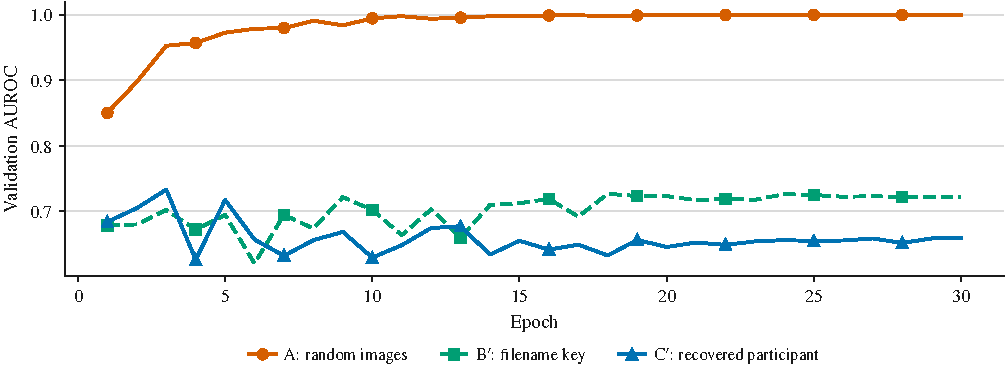
\includegraphics[width=0.85\linewidth]{fig05_learning_curves.pdf}
\caption{Validation AUROC per epoch at seed $= 42$ for Protocol~A
         (random, vermilion), Protocol~B$'$ (filename key, green) and
         Protocol~C$'$ (recovered participant, blue). The vertical
         distance between the first and last curves is the inflation the
         release's own identifier cannot remove.}
\label{fig:learning_curves}
\end{figure*}

\paragraph{Tier-1 takeaway}
Tier~1 is not an independent cohort and we no longer treat it as one: it
is $200$ OASIS-1 participants redistributed without their identifiers.
That makes it the one place in this paper where provenance damage is
observed rather than simulated, and it supplies the quantity the
simulation in \S\ref{sec:provenance_degradation} is calibrated against:
an identifier that is wrong in both directions leaves
\TierOneGapResidual{} AUROC of inflation in place after a correctly
applied subject-wise split. The mechanism behind that inflation is
examined in \S\ref{sec:exp2_probe}, the layer-by-layer decomposition in
\S\ref{sec:exp3_degrad}, and the cohorts with intact identifiers in
\S\ref{sec:exp5_oasis} (OASIS-1) and \S\ref{sec:exp6_adni} (ADNI).

\subsection{Replication on OASIS-1}
\label{sec:exp5_oasis}

We repeat the leaky-versus-\SGA{} comparison on OASIS-1 using the same
ResNet-18 family and the derived 2D slice representation described in
\S\ref{sec:data_oasis}.
Protocol A randomly splits the 1,175 labelled slices by image; Protocol C
uses the frozen subject-component-safe \SGA{} split.
Across five random seeds, Protocol A places nearly every test subject in
training (mean test-subject contamination
\(99.54\% \pm 0.68\%\), range 98.5--100\%).

\paragraph{Why the OASIS-1 gap is mechanically smaller than ADNI's}
Before we report the AUROC numbers, we surface the structural
properties of the OASIS-1 slice manifest that bound the leakage
surface \emph{a priori} (script:
\texttt{scripts/\pb oasis\_subject\_level\_summary.py};
JSON: \texttt{reports/\pb tables/\pb oasis1\_subject\_level\_summary.json}).
Across the labelled subset ($n=235$ subjects with binary
NonDemented/Demented labels; a further $181$ subjects are dropped for
missing CDR at the labelling stage) OASIS-1 has $5$ coronal slices per
session and $2{,}180$ slices across $436$ sessions. Sessions per subject
average $1.05$: only $20$ subjects, $4.8\%$ of the $416$ imaged, carry a
repeat session. Per-subject image
counts are in fact comparable between the two cohorts (OASIS-1
$\approx 5.2$ slices per subject; ADNI1 primary arm $\approx 5.1$
scans per subject at one coronal-centre slice per scan,
\S\ref{sec:data_adni}), so the smaller OASIS-1 gap is not
attributable to a thinner per-subject image stack. The more
plausible mechanism is structural: only $4.8\%$ of OASIS-1 subjects
carry a repeat session, so the cohort contains almost no
longitudinal within-subject variation for a model to exploit,
whereas the ADNI1 cohort is longitudinal by construction. The OASIS-1
replication is therefore best read as a directional replication of
the mechanism, not as a high-powered replication of the inflation
magnitude reported on ADNI (\S\ref{sec:exp6_adni}). The OASIS-1 gap is reported at the image level, and should be read as
the weaker of the two cross-cohort quantities when quoted alongside the
ADNI subject-level result.

% Generated by scripts/gpu_postprocess.py. Do not edit by hand.
\begin{table*}[!tb]
\centering
\caption{OASIS-1 replication: random slice split against the participant-safe \SGA{} split, mean $\pm$ SD over five ResNet-18 seeds at 20 epochs.}
\label{tab:oasis_replication}
\footnotesize
\begin{tabular}{lrrr}
\toprule
\textbf{Metric} & \textbf{Protocol A} & \textbf{Protocol C} & \textbf{Gap (A$-$C)} \\
\midrule
AUROC & $0.828 \pm 0.029$ & $0.793 \pm 0.020$ & \gap{$0.035 \pm 0.037$} \\
Balanced accuracy & $0.712 \pm 0.027$ & $0.704 \pm 0.024$ & \gap{$0.008 \pm 0.043$} \\
F1 (demented) & $0.650 \pm 0.069$ & $0.683 \pm 0.015$ & \gap{$-0.033 \pm 0.076$} \\
Sensitivity & $0.687 \pm 0.225$ & $0.771 \pm 0.137$ & \gap{$-0.084 \pm 0.220$} \\
Specificity & $0.738 \pm 0.174$ & $0.638 \pm 0.179$ & \gap{$0.100 \pm 0.185$} \\
Test subjects leaking & $99.54\%$ & $0\%$ & n/a \\
\bottomrule
\end{tabular}
\end{table*}


The OASIS-1 result (Table~\ref{tab:oasis_replication}) validates the
core leakage mechanism on the cohort Tier~1 was drawn from: the leaky
protocol still places nearly every test subject in the training set
($99.54\%$). While the operating-point metrics (F1, sensitivity) are
statistically noisy across five seeds due to the smaller dataset size,
and one seed produces a negative AUROC gap, the contamination result
confirms that random slice splitting creates severe subject leakage
even when true metadata are available.

\paragraph{DenseNet-121 architecture replication}
Under a DenseNet-121 backbone and the same five seeds the OASIS-1 gap
is \OasisDenseGap{}, mirroring the ResNet-18 result above in point
estimate and in seed-to-seed noise on this small cross-sectional
cohort.

\global\skipbarriertrue
\subsection{Replication on ADNI1, and its robustness arms}
\label{sec:exp6_adni}

We repeat the leaky-versus-\SGA{} comparison on the ADNI cohort
introduced in \S\ref{sec:data_adni}, using the same ResNet-18 family
and coronal-centre-slice representation as
\S\ref{sec:exp5_oasis}. Three split protocols are compared on the same $220$-participant CN-vs-AD
manifest of $1{,}125$ rows, of which $1{,}123$ are diagnosis-resolved.
Protocol~A splits images at random 70/15/15 and is the leaky protocol.
Protocol~B partitions by subject 70/15/15, without the leakage-graph
component, series or near-duplicate constraints. Protocol~C uses the frozen
\SGA{} component-safe split. Test partitions hold $169$, $169$ and $165$
scans respectively, because the component-safe subset-sum assignment cannot
hit the target size exactly. Each protocol
is run for five seeds, 15 epochs each, with AdamW at
$\mathrm{lr}=10^{-4}$ and a class-balanced BCE-with-logits objective.

Under Protocol~A, the random image-level split places nearly every test
subject into the training partition: the mean test-subject contamination
across the five seeds is $99.7\%$, with several seeds reaching
$100\%$. Protocols~B and C, by construction, achieve $0\%$ test-subject
overlap.

% Auto-generated by scripts/generate_adni_paper_tables.py.
% Do not hand-edit; regenerate from the bootstrap JSONs.
\begin{table}[!ht]
\centering
\caption{ADNI inflation gap, 5 seeds, 15 epochs, ResNet-18, coronal centre slice. Numbers are mean AUROC with paired-seed bootstrap 95\% CI (B=10{,}000). ``Test contam.'' = mean \% of test subjects also appearing in the train partition. The MT1-excluded column drops the 28 magnetization-transfer T1 scans for a sequence-homogeneity sensitivity check.}
\label{tab:adni_inflation_gap}
\resizebox{\linewidth}{!}{%
\begin{tabular}{lrrrrrr}
  \toprule
   & \multicolumn{3}{c}{\textbf{All scans (incl. MT1)}} & \multicolumn{3}{c}{\textbf{MT1 excluded}} \\
  \cmidrule(lr){2-4} \cmidrule(lr){5-7}
  Protocol & AUROC [95\% CI] & $n_{\text{test}}$ & Test contam. & AUROC [95\% CI] & $n_{\text{test}}$ & Test contam. \\
  \midrule
  Random (leaky) & 0.947 [0.926, 0.965] & 169 & 99.7\% & 0.960 [0.947, 0.973] & 168 & 99.7\% \\
  Subject-only & 0.837 [0.810, 0.862] & 169 & 0.0\% & 0.833 [0.805, 0.857] & 168 & 0.0\% \\
  Component-safe (\textsc{SplitGuard}) & 0.829 [0.813, 0.846] & 165 & 0.0\% & 0.831 [0.810, 0.855] & 163 & 0.0\% \\
  \midrule
  \multicolumn{7}{l}{\textit{Inflation-gap decomposition (paired bootstrap):}} \\
  Total (random $-$ component-safe) & 0.118 [0.096, 0.145] & & & 0.128 [0.097, 0.159] & & \\
  Subject-leakage (random $-$ subject-only) & 0.110 [0.086, 0.139] & & & 0.127 [0.103, 0.154] & & \\
  Component-marginal (subject-only $-$ comp.-safe) & 0.008 [-0.033, 0.042] & & & 0.002 [-0.017, 0.028] & & \\
  \bottomrule
\end{tabular}}
\end{table}


Table~\ref{tab:adni_inflation_gap} reports the per-protocol test AUROC with
paired-seed bootstrap intervals (B=10{,}000 resamples of
the five-seed array, descriptive;
see ``Statistical conventions'' at the start of \S\ref{sec:experiments}).
The total inflation gap (Protocol~A $-$ Protocol~C) is
\AdniGapTotal{} \AdniGapCI{} AUROC, and the leaky-$>$-\SGA{} direction
holds in all five seeds. A two-level hierarchical
(subject\,$\times$\,seed) re-analysis, the more defensible inferential
quantity, gives \AdniHierGap{} with an interval of \AdniHierCI{} (see
Robustness analyses below). The gap decomposes into a large
subject-identity component (Protocol~A $-$ Protocol~B,
\AdniSubjectPart{}) and a small marginal beyond patient-level
splitting (Protocol~B $-$ Protocol~C, \AdniMarginal{}
\AdniMarginalCI{}) whose interval touches zero.

\paragraph{Subject-level vs image-level evaluation (recommended
clinical reading)}
An image-level AUROC weights participants by scan count, and
participants do not contribute equal numbers of scans. We therefore
aggregate each participant's per-scan predictions (mean
$y_\text{prob}$) and recompute AUROC at the participant level on the
converter-inclusive arm (Table~\ref{tab:adni_subject_level}): the gap
survives the aggregation, and per-protocol AUROC is marginally higher
under it, consistent with within-participant noise reduction. The
image-level number is retained as the cross-cohort-comparable
headline; \emph{but
the subject-level number is the recommended reading for clinical
interpretation}, because it is a stricter aggregation that rules out
per-subject scan-count heterogeneity as a confound and is closer to
the patient-level unit of clinical decision-making. Downstream users
of \SGA{} report cards should quote the subject-level gap in
clinical-adjacent contexts and the image-level gap only in
benchmark-comparison contexts.

% Generated by scripts/gpu_postprocess.py. Do not edit by hand.
\begin{table}[!tb]
\centering
\caption{ADNI image-level against subject-level AUROC on the converter-inclusive arm (five seeds). Both columns are AUROC with a paired-seed bootstrap interval at $B = 10{,}000$. Subject-level numbers average each participant's per-image predictions before computing AUROC.}
\label{tab:adni_subject_level}
\begin{tabular}{lrr}
\toprule
\textbf{Protocol} & \textbf{Image-level} & \textbf{Subject-level} \\
\midrule
Random (leaky) & 0.957 [0.946, 0.969] & 0.966 [0.962, 0.969] \\
Subject-only & 0.789 [0.730, 0.851] & 0.818 [0.771, 0.873] \\
Component-safe (\SGA{}) & 0.815 [0.795, 0.835] & 0.829 [0.794, 0.858] \\
\midrule
\multicolumn{3}{l}{\textit{Inflation gap (Protocol A $-$ Protocol C):}} \\
Image-level & \multicolumn{2}{l}{$+0.142$ [$+0.131$, $+0.158$], positive in 5/5 seeds} \\
Subject-level & \multicolumn{2}{l}{$+0.137$ [$+0.108$, $+0.173$], positive in 5/5 seeds} \\
\bottomrule
\end{tabular}
\end{table}


\paragraph{Robustness analyses}
Four pre-specified arms test whether the headline gap depends on a
particular methodological choice, a fifth row reports the post-hoc
size-balanced control of \S\ref{sec:limitations}, and a sixth isolates
the label-linkage question raised in \S\ref{sec:data_adni}
(Table~\ref{tab:adni_robustness}). All four preserve the
leaky-$>$-\SGA{} ordering in every paired-seed bootstrap resample, and
the total gap moves by at most \AdniArmSpread{} AUROC across them. The
component marginal does not behave that way. It is
$\text{Protocol B} - \text{Protocol C}$ throughout, and it inverts to
\AdniConvMarginal{} on the converter-inclusive arm, opposite to the
direction a leakage-removal effect would take, since there the
component-safe constraints raised AUROC relative to subject-only
splitting rather than lowering it. No interval excludes zero in any arm. We therefore
report the total gap as robust and the component marginal as
unresolved at five seeds, and we do not resolve it by adding seeds.
Two results say why. \S\ref{sec:provenance_degradation} shows the
margin is near-zero on intact cohorts by construction, so the
informative axis is provenance loss rather than seed count; and
\S\ref{sec:permutation_null} measures what a spurious contrast of this
kind looks like at this seed count, finding one of $+0.094$ between two
protocols that had nothing to learn.

% Generated by scripts/gpu_postprocess.py. Do not edit by hand.
\begin{table}[!ht]
\centering
\small
\caption{ADNI robustness arms. The total gap is the paper's headline and the component marginal its null result, measured on the same runs. Intervals are paired-seed bootstrap at $B = 10{,}000$.}
\label{tab:adni_robustness}
\begin{tabular}{@{}lccc@{}}
\toprule
\textbf{Arm} & \textbf{Total gap (A$-$C)} & \textbf{Subject part (A$-$B)} & \textbf{Component marginal (B$-$C)} \\
\midrule
Primary (converters excluded) & $+0.118$ $[+0.096, +0.145]$ & $+0.110$ $[+0.086, +0.139]$ & $+0.008$ $[-0.033, +0.042]$ \\
Converter-inclusive & $+0.142$ $[+0.131, +0.158]$ & $+0.168$ $[+0.105, +0.232]$ & $-0.026$ $[-0.100, +0.048]$ \\
MT1 acquisitions excluded & $+0.128$ $[+0.097, +0.159]$ & $+0.127$ $[+0.103, +0.154]$ & $+0.002$ $[-0.017, +0.028]$ \\
DenseNet-121 backbone & $+0.146$ $[+0.134, +0.161]$ & $+0.136$ $[+0.107, +0.165]$ & $+0.011$ $[-0.026, +0.053]$ \\
Size-balanced assignment & $+0.136$ $[+0.098, +0.159]$ & $+0.110$ $[+0.086, +0.139]$ & $+0.026$ $[-0.040, +0.068]$ \\
\bottomrule
\end{tabular}
\end{table}


The sixth row answers the label-linkage question directly. Restricting
the cohort to the $841$ scans whose diagnosis comes from an exact visit
key, which discards a quarter of the primary arm's scans while keeping
all $220$ participants, gives a total gap of $+0.117$ against the
primary arm's \AdniGapTotal{}, positive on all five seeds, and a component
marginal of $+0.024$ whose interval again spans zero. The headline gap
is therefore not an artefact of the date-matched labels. We put that no
more strongly than the arm supports: dropping a quarter of the scans
widens the interval by nearly half again, from
\AdniGapCI{} to $[+0.072, +0.166]$, so the two point estimates
agreeing to $0.001$ is a coincidence inside overlapping intervals rather
than a precise replication. What the arm establishes is consistency, and
that the date-matched quarter is not carrying the result. The arm also
completes a sensitivity analysis that \S\ref{sec:limitations} could
only run halfway. That one rescored the primary arm's test partition on
its exact-key scans, which tests the labels the gap is measured
\emph{against} while the date-matched scans stay in training; here they
are absent from both sides, and the answer does not change.

The DenseNet-121 arm additionally replicates on OASIS-1
(\OasisDenseGap{}, \S\ref{sec:exp5_oasis}), so the inflation is
consistent in direction across two convolutional backbones on both
source cohorts, though on OASIS-1 neither backbone's hierarchical
interval excludes zero. A two-level subject\,$\times$\,seed
hierarchical resampling widens the total-gap interval on every arm, and
we give all of them rather than only the primary one: \AdniHierCI{}
(primary), $[+0.081, +0.208]$ (converter-inclusive), $[+0.072, +0.191]$
(MT1 excluded), $[+0.087, +0.209]$ (DenseNet-121), $[+0.070, +0.209]$
(size-balanced), $[+0.145, +0.335]$ (volumetric) and $[+0.046, +0.195]$
(exact label linkage). All seven exclude zero. The two OASIS-1 arms are the exception and are reported with the
cross-cohort comparison in \S\ref{sec:exp5_oasis}: $[-0.033, +0.107]$ on
ResNet-18 and $[-0.021, +0.121]$ on DenseNet-121, both spanning zero. Calibration is far worse under
both honest protocols than under the leaky one, and not ordered
between them (Brier/ECE: Protocol~A $0.089$/$0.079$, Protocol~B
$0.247$/$0.253$, Protocol~C
$0.196$/$0.188$)~\cite{niculescu2005calibration,guo2017calibration}:
the leaky protocol is calibrated to its own contaminated test
distribution, which is not a property worth
having~\cite{vancalster2019calibration}. Test-set
demographic composition is balanced by construction across the five
frozen splits (mean $50\% \pm 6\%$ female, $49\% \pm 7\%$ aged
$\geq 76$; $220$ participants, median age 76).

\paragraph{Whole-volume input}
The volumetric arm asks whether the shortcut belongs to the 2D slice or
to the participant. A 3D ResNet-18 on $128^3$ volumes, trained on the
same $220$ participants under the same three protocols, puts the total
gap at \VolGapTotal{} \VolGapCI{}, positive in $5/5$ seeds and
$[+0.145, +0.335]$ under the subject\,$\times$\,seed hierarchical
resampling, against \AdniGapTotal{} on the 2D primary arm. We report
the two side by side rather than as a ratio: the recipes differ in
pretraining and augmentation as well as in dimensionality, so the
comparison establishes that the shortcut survives whole-volume input,
not that volumes leak twice as much. The
gap widens from both ends, and only one of those ends is about leakage.
The leaky level rises to $0.971$, against \AdniRandomAUROC{} in 2D,
which is what a memorisable unit of one whole volume rather than one
slice predicts. The honest level falls to $0.736$, against
\AdniSafeAUROC{} in 2D, and that is not a leakage effect: this network
is trained from scratch on $703$--$723$ volumes per run, where the 2D
arms fine-tune ImageNet features, so its honest performance is not a competitive
volumetric baseline and we do not offer it as one. The transferable
quantity is the gap and not the level, here as everywhere else in this
paper. The decomposition reproduces the 2D pattern: the subject layer
carries the inflation ($+0.268$ $[+0.163, +0.372]$) while the component
layer adds nothing resolvable at five seeds ($-0.033$
$[-0.185, +0.122]$, spanning zero, with subject-only at $0.703$ falling
below component-safe just as it does in the converter-inclusive 2D arm).


\paragraph{Site\,$\times$\,label confound check}
The ADNI CN/AD universe spans 48 recruiting sites (site code extracted
from the first triplet of the ADNI \texttt{PTID}); on the full
universe, uncorrected Cram\'{e}r's $V$ between site and CN/AD label is
$0.36$ ($\chi^2 = 178$, $p < 0.001$), reflecting the well-known fact
that ADNI sites differ systematically in their CN/AD subject mix.
Within the five frozen component-safe \SGA{} splits, this association
is preserved rather than eliminated (script:
\texttt{scripts/\pb site\_scanner\_confound\_audit.py}; JSON:
\texttt{reports/\pb tables/\pb adni/\pb adni\_site\_scanner\_confound\_audit.json}).
Supplementary Table~S7 reports bias-corrected
Cram\'{e}r's $V$ (Bergsma's small-sample correction~\cite{bergsma2013}) for
site$\times$label and sex$\times$label across the five primary-arm
component-safe splits. The site--label association is moderate in
train ($V\approx 0.36$), substantial in validation
($V\approx 0.48$), and strong in test ($V\approx 0.54$, ranging to
$0.72$ across seeds); the sex--label association is negligible in
train and test but reaches $V\approx 0.34$ in the small validation
partition. Scanner field strength is constant across this cohort
and so cannot confound the label. The framework does not perform site-aware
partitioning by design and is therefore not a substitute for site
harmonisation
(ComBat~\cite{johnson2007combat,fortin2017combat,pomponio2020lifespan,bashyam2022deepharmony})
or for explicit site-stratified splitting; the inflation gap we
report is the subject-identity channel that harmonisation does not
fix post-hoc (\S\ref{sec:method}). A site-stratified extension of
the component-safe construction is named as future work in
\S\ref{sec:limitations}.


\begin{figure*}[!tb]
\centering
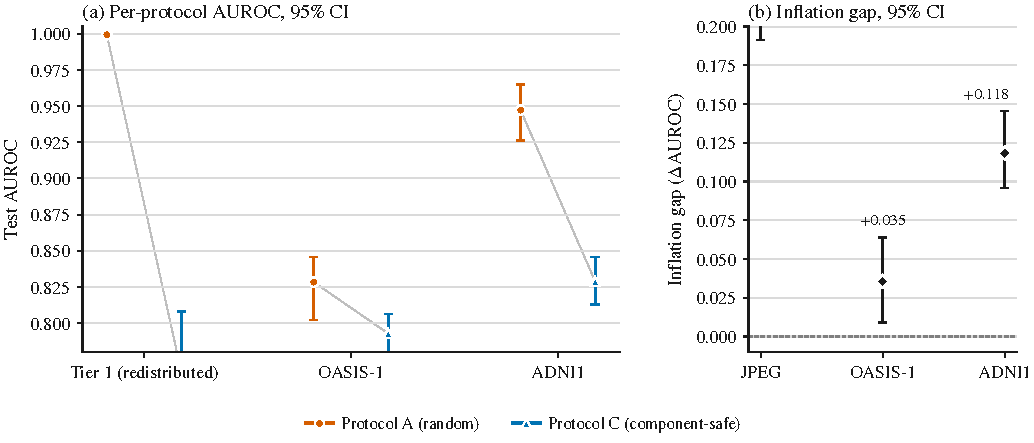
\includegraphics[width=0.95\linewidth]{fig06_cross_cohort_inflation.pdf}
\caption{Direction-preserved inflation gap on the two source cohorts
and on the redistributed benchmark (ResNet-18). (a) Per-protocol test
AUROC (random versus participant-safe) for each cohort; error bars are
paired-seed bootstrap intervals ($B=10{,}000$, $n=5$ seeds per cohort;
descriptive of seed-level variability, see ``Statistical conventions''
in \S\ref{sec:experiments}). Grey lines connect the two protocols
within each cohort. (b) The inflation gap $\Delta\mathrm{AUROC}$ with
the same descriptive intervals. On Tier~1 the participant-safe
protocol is the identity recovered in \S\ref{sec:data_kaggle}, not
the release's own identifier, which is why its gap is larger here than
the one a reader of that benchmark could measure. DenseNet-121
replications are reported in \S\ref{sec:exp5_oasis} (OASIS-1) and
\S\ref{sec:exp6_adni} (ADNI); Tier~1 was run on ResNet-18 only; the figure shows
ResNet-18 for visual parity with the rest of the paper.}
\label{fig:cross_cohort}
\end{figure*}

Figure~\ref{fig:cross_cohort} places the ADNI gap in context under
one reporting convention, paired-seed bootstrap intervals at
$B=10{,}000$. The gap is positive in the mean on both source cohorts:
the small cross-sectional one (OASIS-1, \OasisGapTotal{}
\OasisGapCI{}) and the longitudinal one with substantial repeat
structure (ADNI, \AdniGapTotal{} \AdniGapCI{}). It is positive again,
at \TierOneGapTotal{} \TierOneGapCI{} (hierarchical
$[+0.159, +0.311]$), on the redistribution of the first, where each
participant contributes $32$ slices rather than five. The three differ in how firmly, and we state the difference
rather than averaging over it. On ADNI and Tier~1 the sign holds in
every seed and both the paired-seed and the hierarchical intervals
exclude zero. On OASIS-1 it does not: one of five seeds is negative
($-0.010$), and while the paired-seed interval excludes zero the
subject\,$\times$\,seed hierarchical interval is
$[-0.033, +0.107]$, with the sign preserved in $84\%$ of resamples.
OASIS-1 is therefore a directional replication at the level of the
seed mean, not an independently significant one, and we read it that
way throughout. Patient identity is the dominant leakage channel on
the two cohorts where a subject-only protocol exists to decompose it,
ADNI and Tier~1; OASIS-1 carries no such arm. Subject to that, the
random-split benchmark overstates AD-classification performance by a
magnitude robust to the seed array, the converter-inclusion rule, the
acquisition type, the CNN backbone, input dimensionality and the
strictness of the label linkage.

Figure~\ref{fig:arm_forest} consolidates the headline inflation
results across both source cohorts, the redistributed benchmark, both
backbones and every ADNI robustness arm in a single reporting frame.

\begin{figure*}[!tb]
\centering
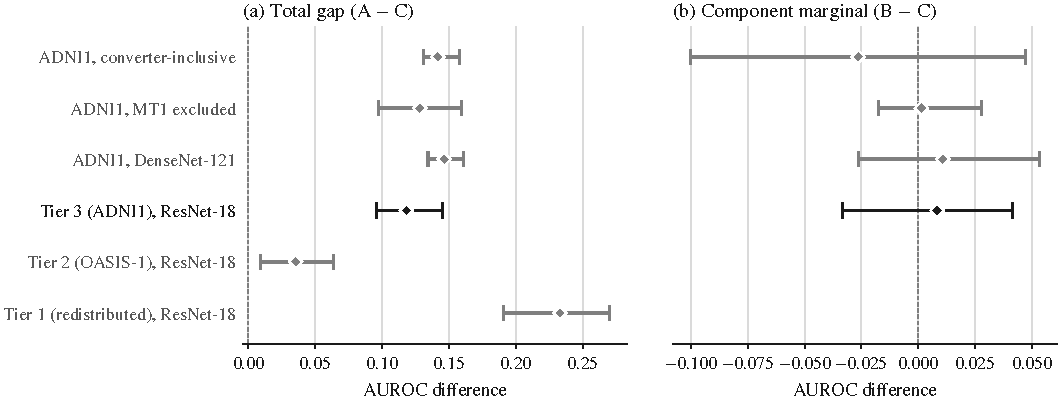
\includegraphics[width=\linewidth]{fig07_arm_forest.pdf}
\caption{The two cross-cohort arms and the six ADNI robustness arms, as
point estimate and paired-seed
bootstrap interval ($B = 10{,}000$, $n = 5$ seeds; descriptive of seed-level variability per the convention in \S\ref{sec:experiments}). The primary arm (Tier~3, ResNet-18) is drawn in black. The volumetric arm is
reported in \S\ref{sec:exp6_adni} and not drawn here, because it
changes architecture, input and training recipe at once and a shared
axis would invite the comparison the text declines. \textbf{(a)} Total gap,
$\Delta\mathrm{AUROC} = \mathrm{Protocol\ A} - \mathrm{Protocol\ C}$.
The per-protocol AUROCs behind each arm are given in the
corresponding subsection; the DenseNet-121 arms reproduce the gap
rather than the absolute level (\OasisDenseGap{} on Tier~2 and
\AdniDenseGap{} on Tier~3).
\textbf{(b)} Component-layer marginal, $\mathrm{Protocol\ B} -
\mathrm{Protocol\ C}$, on its own axis because it is an order of
magnitude smaller. No interval excludes zero and the converter-inclusive
arm inverts; the cross-cohort arms report no marginal and leave the
slot empty. The two panels are the paper's headline and its null result
on the same runs. The ADNI hierarchical (subject\,$\times$\,seed)
bootstrap, the more defensible inferential cross-check, gives gap
\AdniHierGap{}, CI \AdniHierCI{}, direction preserved.}
\label{fig:arm_forest}
\end{figure*}

% ══════════════════════════════════════════════════════════════════════════════

\subsection{Patient reuse manufactures apparent discrimination}
\label{sec:permutation_null}

The gap of the previous section is real and robust, but on its own it
cannot separate ``the leaky protocol learned the disease better'' from
``the leaky protocol recognised its patients''. Both produce a higher
AUROC under random splitting, and no amount of replication across arms
distinguishes them. We separate them by removing the disease.

\paragraph{Design}
Diagnosis labels are permuted across participants and the three protocols
are retrained at the frozen settings, five seeds, $15$ epochs. The
permutation is applied once over the whole cohort rather than inside each
partition, so a participant who straddles a boundary carries the same
permuted label on both sides: within-participant label consistency
survives, the association between anatomy and diagnosis does not. That
detail decides what the control can answer. Permuting inside each
partition preserves per-partition class balance exactly and hands a
straddling participant two different labels, which forecloses identity
memorisation by construction and drives every protocol to chance for a
reason that has nothing to do with the split.

Whether the permutation actually took effect is checked rather than
assumed. Across the scored test rows the permuted label coincides with the
participant's true diagnosis $48.3\%$, $55.1\%$ and $50.3\%$ of the time
under the three protocols. That is the chance rate, and it is the
precondition for reading anything below as patient recall: had the true
labels survived anywhere in the pipeline, the random arm would still score
high and the result would read as a stronger version of the same finding
rather than as a broken one.

\paragraph{Result}
With no disease signal left to learn, the random split still reaches an
AUROC of $0.878$ $[0.837, 0.919]$. The two honest protocols sit at chance:
$0.521$ $[0.427, 0.614]$ under subject-only splitting and $0.427$
$[0.320, 0.533]$ under component-safe splitting, both intervals covering
$0.5$. The seed-paired contrast is $+0.451$ $[+0.357, +0.546]$, positive on
all five seeds.

The training curves say where it comes from. All three protocols drive the
permuted training loss to a comparably low value, $0.068$, $0.037$ and
$0.045$ at the final epoch, so all three memorise the training set about
equally well. Only the random split's memorisation transfers: its final
validation AUROC is $0.863$ against $0.453$ and $0.481$ for the honest
protocols, on a label that carries no information about any image. This is
the shortcut being taken, measured rather than inferred, and it is the
evidence the probe could not supply.

\paragraph{What the number is not}
The permuted gap of $+0.451$ is not the inflation under real labels, which
is \AdniGapTotal{}. It measures the capacity of the memorisation channel
when nothing else is learnable. Under real labels the honest protocols
score around $0.83$ because there is a real signal to learn, and the leaky
protocol's score is bounded above; the channel measured here is one
contributor to that score rather than the whole of it. We report it as
evidence that the channel exists and is large, not as a revised effect
size.

\paragraph{A measured noise floor}
The control also prices the paper's null result. Under permutation the
subject-only and component-safe arms differ by $+0.094$
$[+0.013, +0.175]$, an interval excluding zero, between two protocols that
both have nothing to learn and are therefore both at chance. It cannot
be a difference in what was learned, and its sign has a mechanism worth
naming, because it is not specific to permuted labels. The trainer keeps
the epoch with the best validation AUROC. With the disease signal
removed, the honest arms' validation partitions carry none either, so
that maximum is selection on noise, and the smaller the partition the
further it overshoots: validation optimism, the best validation AUROC
minus the test AUROC, is $+0.007$ under subject-only splitting on a
validation partition averaging $33$ participants, and $+0.159$ under
component-safe splitting on one averaging $22$. The leaky arm shows
$-0.008$ on a validation partition averaging $124$ participants, because
it holds the same patients as training: the signal it selects on is real
memorisation, so there is nothing to overshoot.

Two things follow. A contrast of $+0.094$ arises here between protocols
with nothing to learn, an order of magnitude above the
\AdniMarginal{} component marginal the main experiment reports
(Table~\ref{tab:adni_robustness}), which is why we decline to read that
marginal as an effect and decline to settle it with more seeds of the
same kind. And a component-safe design pays for its safety in
validation size: $22$ participants is too few to select a checkpoint on,
with permuted labels or real ones, which is a cost of the protocol we
had not previously quantified and which any user of it inherits. It is the scale of apparent
protocol-to-protocol difference this design admits at five seeds, and it
is why we decline to read the component marginal as an effect and decline
to settle it by adding seeds of the same kind.



\subsection{Is patient identity decodable, and does that explain the gap?}
\label{sec:exp2_probe}

The permutation control shows the shortcut is taken. A natural next
question is what makes it available, and the answer is a structural
property of the representation rather than anything about the protocol.
A linear probe (LinearSVC) trained on frozen penultimate-layer
features ($512$-dim) of the $15$ ADNI checkpoints of the
converter-inclusive arm recovers participant identity far above
chance, and to the same degree whichever protocol trained the
representation: \ProbeLiftImage$\times$ chance under component-safe
splitting. Holding out a whole visit per participant instead of a
random fifth of their images, so that no repeat acquisition from the
same session sits on both sides, leaves identity decodable at
\ProbeLiftSession$\times$ chance. We run the probe on ADNI rather than
on Tier~1 because ADNI supplies the participant identifiers the probe
classifies; on Tier~1 the release's key is not participant identity
(\S\ref{sec:data_kaggle}).

The interpretation is narrower than the number invites. Identity is
decodable from every one of these representations, including those
trained under honest protocols, so the probe cannot explain a
\emph{difference} between protocols: a quantity that is the same in
both conditions cannot account for the AUROC gap between them. What it
establishes is a structural property of 2D MRI. Repeated slices of one
head share shape, intensity profile and slice position, so identity is
available to any visual representation, and that availability is what
makes test-set contamination exploitable. This also qualifies the
reading that saliency evidence invites: Rumala~\cite{rumala2023}
observes that a leaky network attends to subject-identifying structure
and takes that as the mechanism of the inflation, but identity in the
representation is a precondition for the shortcut rather than evidence
that it was taken. The permutation control of
\S\ref{sec:permutation_null} supplied that evidence by a route needing
no saliency map, and the probe explains why the route exists: identity
is there to be used. The probe uses one architecture and one probe
family; a non-linear adversary in the manner of
DeepBrainPrint~\cite{deepbrainprint2023} or
BrainPrint~\cite{wachinger2015brainprint} would upper-bound it. The
causal weight therefore rests on the three controlled interventions of
\S\ref{sec:permutation_null}, \S\ref{sec:adni_dose_response} and
\S\ref{sec:provenance_degradation}.


\subsubsection{Three-point degradation curve}
\label{sec:exp3_degrad}
The probe answers \emph{whether} identity is encoded; the degradation
curve answers \emph{how much} of the inflation each grouping removes
(Figure~\ref{fig:degradation}).

\begin{figure*}[!tb]
\centering
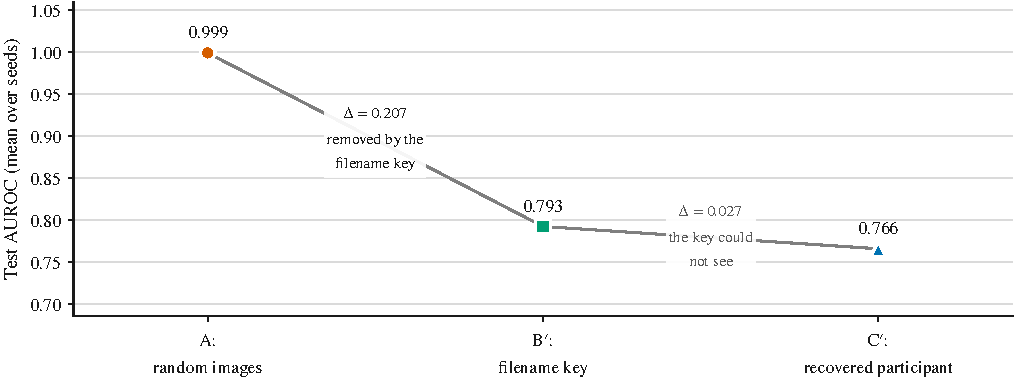
\includegraphics[width=0.82\linewidth]{fig08_degradation_curve.pdf}
\caption{Three-point degradation on Tier~1. Each step changes only
         what the split groups by: random images, then the filename key
         the release ships, then the participant identity recovered
         from OASIS-1. The first step is what an audit run inside the
         release can achieve; the second is what its lost provenance
         hides.}
\label{fig:degradation}
\end{figure*}


The A$\to$B$'$ step is $\Delta$AUROC $=$ \TierOneGapFilename{} and
the B$'\to$C$'$ step a further \TierOneGapResidual{}. On ADNI, where
identifiers are intact, the same decomposition puts
$\sim \AdniShareSubject\%$ of the
gap in the first step. The two cohorts bracket the claim: grouping on
a correct identifier removes most of the inflation, and grouping on a
damaged one does not.

\paragraph{Decomposition takeaway (and head-to-head against
GroupKFold)}
The three-point degradation isolates $\sim \AdniShareSubject\%$ of the ADNI
inflation gap to subject-identity transfer; on Tier~1 the release's
own identifier recovers \TierOneShareFilename\% of the gap, the
remainder being the participants that identifier fails to group
(\S\ref{sec:exp1}). Protocol~B enforces the same
subject-independence constraint as \texttt{GroupKFold}, under a fixed
three-way split rather than $K$-fold cross-validation
(\S\ref{sec:intro}); we did not run \texttt{GroupKFold} itself, so
this decomposition quantifies the marginal value of the
component-safe layer above subject-grouped partitioning rather than
constituting a head-to-head tool benchmark. That marginal, reported throughout as
$\text{Protocol B} - \text{Protocol C}$, is \AdniMarginal{}
\AdniMarginalCI{} on the ADNI primary arm and \AdniConvMarginal{} on
the converter-inclusive arm (Table~\ref{tab:adni_robustness}): small,
of inconsistent sign, and with no interval excluding zero. On Tier~1 the
comparison does not exist in that form, because the release carries no
identifier that Protocol~B could group on.

That marginal should be read with a further caveat that we did not
appreciate until auditing our own splits. Protocols~B and C do not
differ only in their grouping. Protocol~B shuffles participants and
cuts at $70/15/15$ by participant count; Protocol~C consumes a frozen
manifest produced by a size-descending greedy bin-packer that hits
$70/15/15$ by image count. The two therefore differ in the grouping
(the variable of interest) and also in the assignment algorithm
and the quantity the ratios are computed over. On a difference that small, the assignment step is not obviously
negligible relative to the grouping step. The same control failure,
measured directly in \S\ref{sec:provenance_degradation}, was worth
about half the apparent effect there. We therefore report the
component marginal as an upper bound on what the grouping contributes
rather than as an isolated estimate of it, which reinforces rather
than weakens the conclusion already stated: the marginal is small, of
inconsistent sign, and not resolved.

The greedy also leaves a visible fingerprint on the frozen ADNI
manifests. Because it fills the validation and test bins first and
takes the largest components that still fit, the partitions end up
nearly disjoint in component size: across the five seeds, training
components span $4$--$6$ scans (mean $4.65$), validation $7$--$9$
(mean $7.50$) and test $5$--$7$ (mean $6.11$). Participants with
longer longitudinal records are systematically routed away from
training. Class balance survives this, because components are
stratified by label before the subset-sum assignment runs ($39.1\%$, $38.2\%$
and $40.0\%$ AD by image across the three partitions), but within each
class the test partition is enriched for participants with more
follow-up. That matters clinically: in this cohort AD participants
contribute fewer scans than CN participants ($4.55 \pm 0.97$ against
$5.56 \pm 1.00$), so scan count tracks retention, and retention tracks
disease course. This is an instance of the duration-dependent
selection bias described in the data-handling
literature~\cite{rouzrokh2022mitigating}, arriving through the
splitter rather than through the cohort.

We do not leave this as a caveat. The frozen manifests are retained
because every number in this paper is computed on them and exact
reproducibility is worth more than a cosmetic correction, but a
size-balanced split was generated specifically to test whether the
headline result depends on the defect. Visiting components in shuffled rather than size-descending order removes
the stratification. Mean component sizes become $5.15$, $5.00$ and $5.07$
scans in train, validation and test, against $4.65$, $7.50$ and $6.11$ on
the frozen split. The total gap is \SizeBalancedGap{} on the size-balanced
split against \AdniGapTotal{} on the frozen one, with hierarchical intervals
$[+0.070, +0.209]$ and \AdniHierCI{}. We report it beside the primary arm
rather than after it. The composition defect is real, it was found by this
project's own audit of its own splits, and the effect it was suspected
of producing is not there. What it does mean for the audit gate, which
passed this split on every check it performs, is taken up in
\S\ref{sec:limitations}.

The dominant practical
recommendation is therefore straightforward and not novel, split by
subject identity. The leakage-graph machinery (component-level and
near-duplicate edges) costs essentially nothing on cohorts with clean
participant identifiers, and buys nothing measurable there either: we
claim no \emph{AUROC} benefit from it on ADNI or OASIS-1.
\S\ref{sec:provenance_degradation} shows what it does buy, on the axis
where it can: structural protection against patient leakage once
subject identifiers start disappearing. We can, however, exhibit the failure mode
it exists for, which the next paragraph does. We retain the
component-safe construction as the conservative default in the
pre-training GO/NO-GO gate; readers running the framework on cohorts
where subject identity is clean and converter-free should expect the
component-safe and subject-only protocols to be statistically
indistinguishable. The honest contribution claim is therefore
infrastructural (an executable AD-specific audit with a binary
gate), not that the component-graph layer outperforms a careful
subject-aware GroupKFold on every cohort.

\paragraph{Where grouping by the available identifier is blind}
\label{sec:subject_inference_failure}
Subject-wise splitting can only protect images whose participant is
known, and a redistributed benchmark is exactly the case where that
premise fails without saying so. Tier~1 makes the failure measurable,
because its true identities are recoverable from outside the release
(\S\ref{sec:data_kaggle}), which is not something its users have.

The exposure is not a handful of edge cases but the structure of the
release, measured in \S\ref{sec:data_kaggle}: a key that merges and
splits participants, images with no key at all, and a split that every
check the release supports calls clean while most of its test set is
contaminated. This is the regime the component layer exists for, and
the honest reading of Tier~1 is that the layer does not rescue it
either, because the redistribution removed the session and series
identifiers the graph would have carried. The consequence for a reader
of public benchmarks is stronger than a recommendation to split by
subject: where a release does not document provenance, a subject-wise
split of it cannot be verified from inside the release at all, and the
number it reports cannot be interpreted.

\subsection{What the gap costs at a screening operating point}
\label{sec:adni_subgroup}

Running both leaky and honest protocols on the same ADNI universe is
not just a robustness check; it surfaces \emph{two} findings that the
leaky benchmark would have concealed. First, a sex-related performance
disparity emerges under both honest protocols and collapses to
indistinguishable from zero under the leaky one
(Supplementary Material~S6). Sex differences in AD are well documented: in atrophy rates on ADNI
itself~\cite{hua2010sex}, in verbal-memory reserve that can delay
diagnosis in women~\cite{sundermann2016female}, and in incidence and
prevalence~\cite{mielke2014clinical}, so a protocol that conceals a
performance disparity between sexes conceals something the clinical
literature says should be looked for. We report ours as exploratory
and do not attribute it to any of these mechanisms. Second, the AUROC gap translates into
a concrete clinical cost-of-leakage at the screening operating point
that a clinician trusting the leaky number would systematically
underestimate (\S\ref{sec:adni_cost_of_leakage}). Both findings rely on
the per-image test predictions persisted by the converter-inclusion
sensitivity arm; both rely on the framework's audit-and-prevent design
to render them visible.

\subsubsection{Cost-of-leakage as an arithmetic illustration}
\label{sec:adni_cost_of_leakage}
To express the gap in units a clinician can weigh, we re-expressed the
sensitivity difference at a fixed screening specificity of $0.90$ as
missed-diagnosis counts per $1{,}000$ screened, under literature-cited
prevalence anchors. Sensitivity at that specificity is $0.866 \pm 0.046$
under Protocol~A against $0.535 \pm 0.103$ under Protocol~C, which at the
US 75--84 population prevalence of $13.8\%$~\cite{rajan2021} is
\MissedPerThousand{} additional missed AD cases per $1{,}000$ screened if
the leaky benchmark is trusted.

This is deterministic arithmetic applied to the measured sensitivities, not
a deployment estimate. It inherits every cohort caveat in
\S\ref{sec:limitations}: a single 2D coronal-centre slice, a research cohort
that is not a screening population, a threshold chosen on validation, and no
prospective evaluation. We give it because an AUROC difference is hard to
weigh and a count is not, and we give it once. The operating-point
derivation, the sensitivity of the result to the chosen specificity, and the
second prevalence anchor are in Supplementary Material~S2.

\subsection{Leakage as a dose: injecting test-set overlap}
\label{sec:adni_dose_response}

The cross-tier inflation gap and the cost-of-leakage translation both
take the leakage condition as binary (leaky vs.\ honest). A more
informative question for benchmark designers is the dose-response: if
$p\%$ of test subjects also appear in train, how much AUROC inflation
should we expect? We answer this with a controlled stress-test on
the converter-inclusive ADNI sensitivity arm.

\paragraph{Design}
Starting from the Protocol~C component-safe split, we generate a family
of injected splits at target contamination fractions
$p \in \{0, 0.25, 0.50, 0.75, 1.0\}$, where \emph{$p$ is the share of
test scans that belong to a training participant}, not the share of
test participants. For each non-zero $p$ we draw
$k = \lfloor p \cdot 258 \rceil$ participants from the multi-visit
training subset and substitute one alternate scan of each into the test
set, displacing an equal number of original test scans. Because each
donor contributes a single scan, the share of contaminated test
\emph{participants} is never smaller and is usually far larger ($63\%$,
$77\%$ and $86\%$ of test participants at $p = 0.25$, $0.50$ and
$0.75$, converging to equality only at $p = 1$), which is why every
composition below is done in scan units. Class
balance of the \emph{injected partition} (118~CN $/$ 140~AD over $258$
rows) is held fixed at every overlap level by stratified substitution.
The partition the model is \emph{evaluated} on is not held fixed either,
and this qualifies the calibration. The binary pipeline drops MCI scans and
substitution displaces them, so the evaluated CN/AD subset grows from $203$
rows at $p=0$ to $258$ at $p=1$, with the AD share rising from $47.7\%$ to
$54.3\%$. These are five-seed means; the $p=0$ count runs from $197$ to
$207$ across seeds.

The training partition is not held fixed either, and this is the more
consequential of the two. Each substituted scan is moved out of training,
so evaluated training rows fall from $1{,}041$ at $p=0$ to $783$ at
$p=1$, $24.8\%$ of them, as the dose rises. The donor
\emph{participant} remains in training, which is why donors are drawn only
from the multi-visit subset, so the identity leakage the arm is built to
create is genuine; what the arm does not do is hold the training set
constant while adding it.

The dose axis is therefore confounded with both test composition and
training size, and the two plausibly act in opposite directions: thinning
the training set should depress AUROC at high $p$, while the class
enrichment above has no clear sign. The slope is consequently descriptive
of this substitution procedure as a whole, and is not a causal price per
unit of realised leakage. Both quantities are measured by
\texttt{scripts/\pb analyze\_dose\_response\_composition.py} and reported in
\texttt{reports/\pb tables/\pb adni/\pb adni\_dose\_response\_composition.json}. We report it rather than correct it
because the two cannot be separated without changing the injection
mechanism, and because the two cannot be separated without changing the
mechanism: the slope is used only as a floor
(\S\ref{sec:adni_cost_of_leakage}). Otherwise this is biometric-identity
leakage alone: no slice or near-duplicate is shared between train and
test, only the patient. We run the full $5\text{ seeds} \times 5\text{ overlaps}$
matrix on two architecture families (ResNet-18 and DenseNet-121,
$15$ epochs each, $\mathrm{lr}=10^{-4}$ AdamW), a total of $50$
training runs.

\paragraph{Result}
Figure~\ref{fig:dose_response}(a) shows the resulting per-seed AUROCs
and the seed-averaged dose-response curves with $95\%$ paired-bootstrap
CIs. The seed-averaged curves increase with test-subject overlap for
both architectures; per-seed monotonicity holds in $5/5$ ResNet-18 seeds
but in $0/5$ DenseNet-121 seeds (Supplementary~S4);
the fitted ResNet-18 endpoints
(\DoseAtZero{} at $p=0$, \DoseAtOne{} at $p=1$) sit within $0.02$ of
the converter-inclusive arm's honest and leaky levels
(\AdniConvSafeAUROC{} and \AdniConvRandomAUROC{},
\S\ref{sec:exp6_adni}), which is the arm the injected splits are built
from. We read that agreement as a sanity check and not as a
calibration: the matrix and those levels come from the same code state
on different GPUs (\S Declarations), and nothing in the injection was
tuned to reproduce them. The straight-line OLS fit
(Figure~\ref{fig:dose_response}(b)) recovers
\begin{equation}
\widehat{\mathrm{AUROC}}_{\text{ResNet-18}}
   = \DoseIntercept{} + \DoseSlope{} \cdot p, \qquad R^2 = \DoseRSq{},
\label{eq:dose_response}
\end{equation}
and a similar but noisier curve for DenseNet-121
($\widehat{\mathrm{AUROC}} = \DoseDenseAtZero{} + \DoseDenseSlope{}
\cdot p,\ R^2=0.64$).
The slope of $+\DoseSlope{}$ AUROC per unit overlap on
ResNet-18 implies a cohort- and architecture-specific calibration
point: on this ADNI universe and this 2D-slice representation, every
$10$ percentage points of test-subject overlap inflates the reported
AUROC by approximately $+0.013$. The point-estimate predictions from
Equation~\ref{eq:dose_response} are usefully read as the
deterministic part of a noisy calibration; the per-seed scatter
around the regression line in
Figure~\ref{fig:dose_response}(b) is approximately consistent with an
additive Gaussian residual, so the dose-response can equivalently be
written
\begin{equation}
\mathrm{AUROC}(p) \;=\; \alpha + \beta \cdot p \;+\; \varepsilon,
\qquad \varepsilon \sim \mathcal{N}(0, \sigma^2),
\label{eq:dose_response_noisy}
\end{equation}
with $(\widehat{\alpha},\widehat{\beta}) = (\DoseIntercept{}, \DoseSlope{})$ and
$\widehat{\sigma} = 0.0191$ on ResNet-18 ($0.0250$ on DenseNet-121),
the residual standard deviation of the twenty-five per-seed
observations about the OLS fit. The unit matters: because the band is
meant to describe a \emph{single} training run, it has to be estimated
from single runs. Taking it instead from the five per-overlap means
would give $0.008$ and understate the spread roughly $2.5$-fold, since
averaging five seeds removes most of the seed-level variance the band
exists to represent. So estimated, $\widehat{\sigma}$ gives an
order-of-magnitude prediction band for one run at a given $p$ and lets
the equation be used probabilistically (\eg{} the probability that a benchmark reporting
AUROC $A$ at measured contamination $p$ exceeds its true
component-safe value by more than $0.05$ can be estimated from the
upper tail of $\mathcal{N}(A - \widehat{\alpha} - \widehat{\beta}p,\
\widehat{\sigma}^2)$).
We report the OLS slope as a descriptive calibration constant rather
than as an inferential coefficient (the twenty-five $(\text{seed},
\text{overlap})$ observations are not independent under OLS). A
random-intercept model fitted by iterated feasible GLS under compound
symmetry gives the same slope, $\widehat{\beta} = 0.1251$, because the
design is balanced; what changes is the interval. With a
cluster-robust sandwich standard error carrying the finite-cluster
correction and a $t(4)$ critical value, the $95\%$ CI is
$[0.0866, 0.1636]$ on ResNet-18; DenseNet-121 gives
$\widehat{\beta} = 0.0906$ with $95\%$ CI $[0.0416, 0.1396]$. Both
exclude zero. Full specification, the fitted variance ratio, the
seed-cluster bootstrap, and Spearman monotonicity statistics are in
Supplementary Material~S4. Density-choice
qualifications and finer-grid trade-offs are discussed in
\S\ref{sec:limitations}.

\begin{figure*}[!tb]
\centering
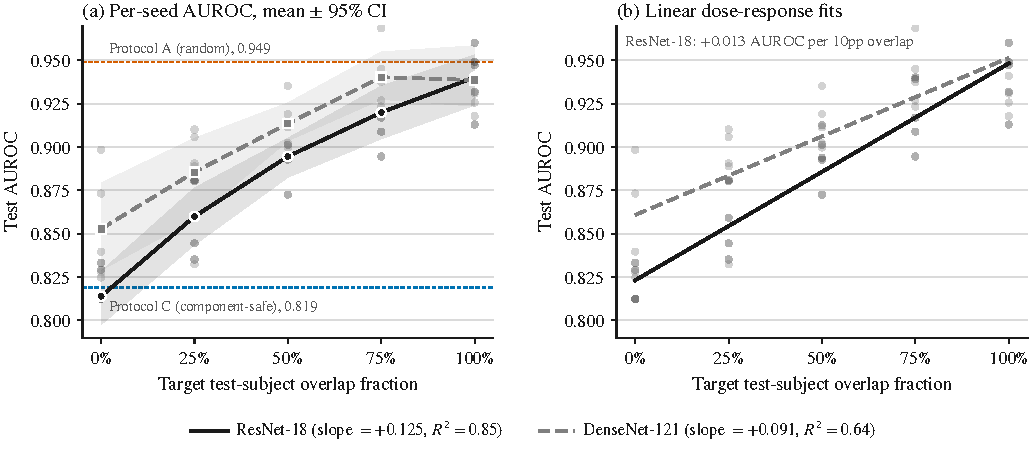
\includegraphics[width=0.98\linewidth]{fig11_dose_response.pdf}
\caption{ADNI leakage dose-response on the converter-inclusive
sensitivity arm. (a) Per-seed test AUROCs (small dots), seed-averaged
mean (markers + line) and $95\%$ paired-bootstrap CI band for each architecture as a function of the target test-subject overlap fraction $p$; ResNet-18 is drawn in black and DenseNet-121 in grey (dashed), and the reference lines take the colour of the protocol they mark. Reference lines mark the \emph{primary-arm} Protocol~C
component-safe baseline (\AdniSafeAUROC{}) and Protocol~A leaky
benchmark (\AdniRandomAUROC{}) from \S\ref{sec:exp6_adni}, shown for
cross-arm comparability. The matrix itself is built on the
converter-inclusive arm, whose own levels are \AdniConvSafeAUROC{} and
\AdniConvRandomAUROC{}; the fitted endpoints are \DoseAtZero{} and
\DoseAtOne{} (panel a).
(b) OLS linear fits to the per-seed points show the dose-response slope;
the ResNet-18 slope of $+\DoseSlope{}$ AUROC per unit overlap is a cohort- and
architecture-specific calibration point on this ADNI universe and this
2D-slice representation, not a claim that the slope generalises to
other cohorts or 3D representations.}
\label{fig:dose_response}
\end{figure*}

\paragraph{Interpretation}
The dose-response is approximately linear over the entire $[0,1]$
overlap range, with one qualification we state rather than smooth
over: the ResNet-18 increments shrink monotonically across the sweep
($+0.046$, $+0.035$, $+0.025$, $+0.020$) and the DenseNet-121 mean
falls slightly at the last step ($0.9403$ at $p=0.75$ to $0.9387$ at
$p=1$). That is a mild saturation as the leaky endpoint is approached,
which is what a bounded metric does near its ceiling, and not a
threshold below which contamination is harmless. No threshold effect
appears anywhere in the range, which is consistent with the
biometric-probe finding
(\S\ref{sec:exp2_probe}) that subject identity is encoded as a
roughly continuous signal in 2D MRI representations. Both
architectures' $p=1$ endpoints converge near the Protocol~A leaky
AUROC, as expected: $100\%$ subject overlap is mechanically
equivalent to the random-split condition. The DenseNet-121 curve has
a higher baseline AUROC at $p=0$ ($0.853$ vs.\ $0.814$) and a flatter
slope ($+\DoseDenseSlope{}$ vs.\ $+\DoseSlope{}$). The two mixed-effects slope
intervals overlap ($[0.0866, 0.1636]$ vs.\ $[0.0416, 0.1396]$;
Supplementary~S4) and we run no formal difference test, so the two
architectures' dose-response slopes are not distinguishable at five
seeds and we draw no inference about backbone capacity. The DenseNet $R^2$ of $0.64$ still
trails the ResNet-18 fit, and no DenseNet seed is monotonic across all
five overlaps: with five seeds per overlap and a smaller endpoint
separation, the trend is carried by the seed average rather than
visible within any single seed.

\paragraph{Practical use, and why the slope is a floor}
Equation~\ref{eq:dose_response} converts a measured test-subject
contamination fraction
(which the pre-training audit already reports) into expected AUROC inflation. It should be read as a lower bound
on the gap rather than as an estimate of it, for a reason that follows
from how it was fitted: the injection varies test-subject overlap by
substitution, so it prices the participant-identity channel and no other,
while thinning the training set as it does so. A naive split on a real cohort additionally leaks
through slices of one volume, near-duplicates and re-acquisitions, none
of which the slope sees.

Two of the three cohorts bear this out, and the third does not; we give
all three rather than the two that agree. Under random splitting,
contamination is essentially complete on every one: on ADNI1 because
participants contribute about five scans each, on Tier~1 because a
participant's $32$ slices are all but certain to land on both sides of
the split, and on OASIS-1 where $99.5\%$ of test subjects also appear in
training. The equation therefore predicts a drop of
at most $\DoseSlope{}$ on each, against a measured \AdniConvGap{} on the
converter-inclusive ADNI1 arm the injected splits are built from and
\TierOneGapTotal{} on Tier~1, and the larger shortfall on Tier~1
is what one would expect where adjacent slices of one volume add a
channel the slope does not price. On the converter-excluding primary
arm the measured gap is \AdniGapTotal{}, which the predicted floor now
matches to within $0.01$. OASIS-1 is the case that does not fit: its
contamination is as complete as the others' yet its gap is
\OasisGapTotal{}, roughly a third of the predicted floor, so on that
cohort the floor is not a floor. We take this as the boundary of the
calibration rather than a refutation of it: OASIS-1 contributes five
slices per participant from a single cross-sectional visit, so a
contaminated test image resembles its training counterpart far less than
a repeat visit of the same ADNI participant does, and the slope was
fitted where repeat structure is the dominant form of overlap. The
margin the floor leaves is therefore a property of
the cohort it is applied to, not a guarantee, and on a cohort whose
identity channel is the whole of its leakage the floor is the estimate. Used as a point estimate the
equation would tell a reader their honest AUROC is higher than it is,
the wrong direction to err in for a quantity whose purpose is to
correct over-reporting. Used as a floor it answers the question worth asking of
a benchmark: whether the contamination present is large enough to
matter at all.


% ------------------------------------------------------------------------------
\subsection{Provenance loss: what the leakage graph buys when identifiers fail}
\label{sec:provenance_degradation}

\S\ref{sec:leakage_graph} reports that on every cohort studied here the
connected components coincide exactly with a subject grouping, so the
component layer earns nothing over \texttt{GroupKFold}-style splitting.
That is a consequence of subject being the coarsest identifier: session,
series and acquisition-date edges all nest inside it, so none of them can
change a component while \texttt{subject\_id} is present and correct. The
framework's stated scope condition is therefore that the extra edge
families matter only where subject identity is absent, corrupted, or
inferred wrongly. Until now that was an assertion. This section measures
it.

\paragraph{Design}
The regime is created deliberately, using the same template as the
dose-response experiment in \S\ref{sec:adni_dose_response}: hold
everything fixed, sweep one controlled quantity, read off the curve. Here
the swept quantity is provenance loss. Starting from the ADNI1 primary
arm, where subject identifiers are complete and authoritative, we delete
\texttt{subject\_id} on a random $0/10/25/50/100\%$ of scans and ask what
each protocol does with the remainder. Deletion is applied per scan
rather than per subject because that is the observed failure mode:
redistributed benchmarks lose the patient index one filename at a time,
so a record is typically partly recoverable rather than wholly anonymous.
Under Protocol~B every scan whose identifier was removed becomes its own
group and may be placed in any partition. Under Protocol~C the leakage
graph is rebuilt from whatever identifiers survive; \texttt{session\_id}
and \texttt{series\_uid} are globally unique on this cohort ($1{,}003$
and $1{,}008$ distinct values, no blanks, and no value shared between two
participants) and do not take \texttt{subject\_id} as an input, so they
continue to bind scans that \texttt{same\_subject} can no longer reach.

The outcome is scored against the untouched ground-truth identifiers,
which the degradation preserves out of band. We report the number of true
participants with scans on both sides of a partition boundary. This is a
structural measurement: it counts the leakage each protocol actually
admits without routing the question through a trained model, and it is
therefore free of the seed-variance and test-set-size caveats that
qualify the AUROC comparisons elsewhere in this paper.

\begin{table*}[!tb]
\centering
\small
\caption{Provenance degradation on the ADNI1 primary arm ($220$
participants, five seeds, mean\,$\pm$\,SD). Columns report participants
whose scans straddle a partition boundary, and $p$, the fraction of
test-partition participants who also appear in training, the same quantity the dose-response experiment sweeps, so the two curves compose.
At zero loss the protocols are identical, which is the
\S\ref{sec:leakage_graph} null result restated as the origin of a curve
rather than as a dead end.}
\label{tab:provenance_degradation}
\begin{tabular}{@{}lrrrr@{}}
\toprule
\textbf{Identifiers} & \multicolumn{2}{c}{\textbf{Straddling participants}}
                     & \multicolumn{2}{c}{\textbf{$p$ (test\,$\cap$\,train)}} \\
\cmidrule(lr){2-3}\cmidrule(lr){4-5}
\textbf{deleted} & Protocol B & Protocol C & Protocol B & Protocol C \\
\midrule
$0\%$   & $0.0 \pm 0.0$   & $0.0 \pm 0.0$   & $0.000$ & $0.000$ \\
$10\%$  & $18.6 \pm 5.0$  & $9.4 \pm 1.9$   & $0.361$ & $0.207$ \\
$25\%$  & $31.4 \pm 3.1$  & $19.8 \pm 2.0$  & $0.374$ & $0.408$ \\
$50\%$  & $77.0 \pm 5.0$  & $53.6 \pm 6.6$  & $0.980$ & $0.807$ \\
$100\%$ & $182.6 \pm 7.2$ & $125.4 \pm 1.3$ & $0.993$ & $0.990$ \\
\bottomrule
\end{tabular}
\end{table*}

\begin{figure*}[!tb]
\centering
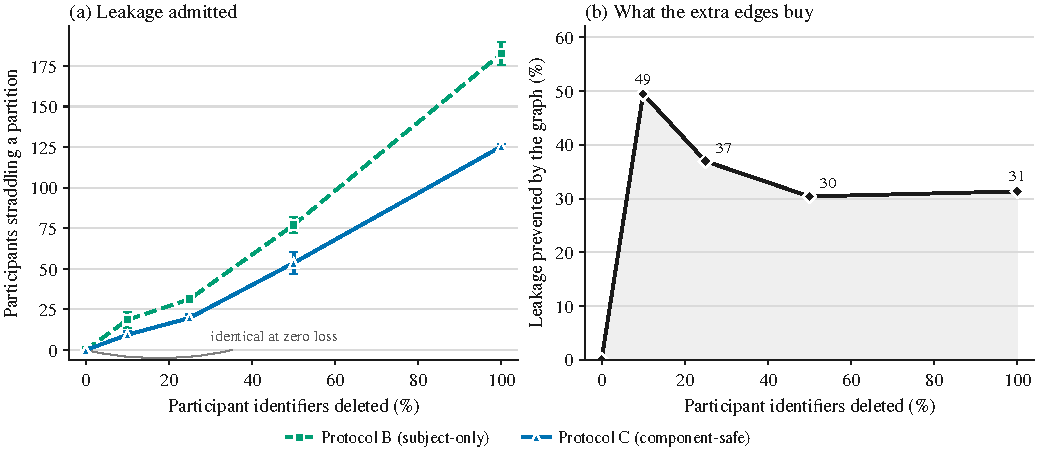
\includegraphics[width=\linewidth]{fig12_provenance_degradation.pdf}
\caption{Provenance degradation on the ADNI1 primary arm, five seeds,
mean\,$\pm$\,SD. \textbf{(a)} Participants whose scans straddle a partition
boundary as participant identifiers are deleted. This counts admitted leakage
directly, without routing the question through a trained model. The two
protocols are indistinguishable at zero loss
(the equivalence reported in \S\ref{sec:leakage_graph}, here the origin
of a curve rather than a dead end) and separate immediately thereafter. \textbf{(b)} The share of that leakage
the leakage graph prevents. Both protocols use the same assigner, so the
difference is attributable to the grouping; under a mismatched assigner the
$10\%$ figure reads $78\%$. The benefit peaks in the regime where
redistributed benchmarks sit and decays once too few identifiers survive for
any rule to bind on.}
\label{fig:provenance_degradation}
\end{figure*}

\paragraph{Result}
Figure~\ref{fig:provenance_degradation} and
Table~\ref{tab:provenance_degradation} give the curve. At zero loss
the two protocols admit no leakage and are indistinguishable,
reproducing the equivalence reported in \S\ref{sec:leakage_graph}.
They separate immediately thereafter: at $10\%$ identifier loss the
leakage graph prevents $49\%$ of the participant leakage subject-wise
splitting admits ($9.4$ versus $18.6$ straddling participants), and
$30$--$37\%$ at higher loss rates.

Both protocols are assigned by the same class-stratified bin-packer
over their respective groupings, so the difference is attributable to
the grouping and not to the assignment step. That control matters more
than it may appear. An earlier version of this comparison assigned
Protocol~B by shuffling subject groups and cutting at $70/15/15$ by
group count, while Protocol~C bin-packed by image count; under that
mismatched design the graph appeared to prevent $78\%$ of residual
leakage at $10\%$ loss. Roughly half of the apparent benefit came from
the assigner rather than from the grouping. We report the matched
comparison because only the grouping is the claim.

\paragraph{Provenance loss amplifies non-linearly}
Deleting $10\%$ of identifiers returns $36\%$ of test participants to
the training partition under Protocol~B, a roughly threefold
amplification. The mechanism is elementary once stated: a participant
contributes a median of five scans, and one of them losing its index
is enough to detach that scan from the group and let it land opposite
the other four. Participant-level protection is not degraded
gracefully by scan-level provenance loss; the first missing identifier
in a record breaks it.

\paragraph{Composing the two curves, and where the composition fails}
Chaining the two curves requires them to share a unit. The injection
experiment sweeps the share of contaminated test \emph{scans}, so that
is the quantity we compose through: at $10\%$ identifier loss it is
\ProvScanTenSubject{} under Protocol~B and \ProvScanTenSafe{} under
Protocol~C, against \ProvParticipantTenSubject{} of test
\emph{participants} under Protocol~B. Read through
Equation~\ref{eq:dose_response}, that is $+\ComposedTenSubject{}$ AUROC
of expected optimism under Protocol~B against $+\ComposedTenSafe{}$
under Protocol~C. That composition under-predicts what the same
experiment measures directly, and the comparison is worth stating
because it bounds how much weight the chain carries: the provenance arm
itself trains at every deletion level, and its test AUROC rises from
$0.771$ at no loss to \ProvSubjectAUROCTen{} under subject-wise splitting
and \ProvSafeAUROCTen{}
under the component-safe protocol at $10\%$ loss, that is $+0.095$ and
$+0.059$ against the two composed figures just given. The chain is low
by rather more than a factor of two in both protocols. Two reasons are visible: the slope is fitted on
a cohort whose contamination is varied by substitution, which thins
training as it adds overlap, whereas deleting identifiers perturbs both
sides differently, and the slope
and the shares come from different arms of one code state
(\S Declarations). We therefore read the composition as an order of
magnitude and a lower bound, never as a coefficient, and we report the
directly measured rise beside it rather than only the chain. Table~\ref{tab:provenance_degradation} reports the
participant share $p$ alongside it, because that is what a split audit
shows a reader.

We do not present that as a general result, because $p$ is not
monotone across the sweep. At $25\%$ loss Protocol~C's $p$ ($0.408$)
exceeds Protocol~B's ($0.374$), inverting an ordering that holds at
every other level and that the straddling-participant count preserves
throughout. The reason is that $p$ is a ratio whose denominator is the
number of distinct test participants, and the two protocols do not
produce test partitions containing the same number of them:
component-safe grouping yields larger and fewer components, hence a
smaller and differently composed test partition. $p$ is therefore a
defensible input to the dose-response fit, where it is measured within
a single protocol, but a poor instrument for comparing protocols. The
straddling-participant count, which counts events rather than ratios,
does not have that defect, and it is the measurement the result above
rests on. We give the composition at $10\%$ as an illustration of what
chaining the two experiments would yield, and explicitly not as a
validated protocol-level comparison.


\paragraph{Scope}
Three limits belong with this result. The measurement is primarily structural: it counts admitted leakage,
and the AUROC arm trained on the same degraded manifests is reported
in \S\ref{sec:limitations} rather than here. The degradation is synthetic, imposed on a
cohort with complete provenance rather than observed on one that lost it,
which is what makes ground-truth scoring possible and also what makes it
a model of the failure rather than the failure itself. And the recovery
depends on which identifiers a cohort happens to carry: ADNI1 supplies
globally unique session and series keys, whereas the Tier-1 benchmark
supplies neither, so the curve measured here is an upper bound on what
the same protocol could achieve on a cohort stripped down to filenames.

\subsection{Structured provenance corruption: where the graph earns its place}
\label{sec:provenance_stress}

The deletion experiment removes identifiers \emph{visibly}. A missing
\texttt{subject\_id} is a value a splitter can see is absent, and the honest
response, treating that scan as its own group, is available to any
\texttt{GroupKFold} user. Redistribution rarely fails that politely. The
Tier-1 benchmark in \S\ref{sec:exp1} carries a key for every image and the
key is simply wrong: it splits $179$ of $200$ participants across several
keys and merges others under one. Nothing is missing, so nothing looks
broken.

\paragraph{Design}
We therefore apply a corruption operator
$C \in \{\textsc{drop}, \textsc{split}, \textsc{merge}\}$ at intensity
$\lambda$ to the ADNI1 primary manifest, rebuild both groupings on the
corrupted result, and score residual leakage against untouched ground truth.
\textsc{drop} removes a scan's identifier with probability $\lambda$;
\textsc{split} deals a participant's scans into two pseudo-identifiers with
probability $\lambda$, so one patient looks like two; \textsc{merge}
relabels a random pair of participants to one pseudo-identifier, so two
patients look like one. The last two mimic the observed Tier-1 failure modes
and leave no field missing. These operators are controlled stress tests
of identifiable provenance failure modes; they are not estimates of the
prevalence or the distribution of such errors in clinical repositories,
and we draw no conclusion about how often real cohorts sit at any given
intensity. Only the grouping differs between the protocols
compared; both use the same class-stratified assigner, for the reason given
above. The experiment has two halves, and only the second needs a GPU.
Contamination is a property of the split, so the leakage every cell admits
is measured without fitting anything; the AUROC each corrupted split then
produces is measured by training one model per protocol per seed, $120$
models in all.

\paragraph{Result}
Table~\ref{tab:stress_structural} gives the matrix. The three mechanisms
separate cleanly, and one of them is where the component
layer stops being redundant. Under \textsc{drop} the graph halves the damage
at $\lambda = 0.1$ ($16.8$ straddling participants under subject-wise
grouping against $8.4$), falling to $31\%$ prevented at total loss, which
reproduces \S\ref{sec:provenance_degradation} by a second route. Under
\textsc{split} it prevents $50\%$ at $\lambda = 0.1$ (a small absolute
effect at that intensity, $1.2$ straddling participants against $0.6$)
and $90\%$ at
$\lambda = 1$, where subject-wise grouping admits $61.6$ straddling
participants and the graph admits $6.4$, with test-scan contamination falling
from $64\%$ to $11\%$. That gap is the framework's reason to exist: when one
participant is dealt into two keys, \texttt{same\_session},
\texttt{same\_series\_uid} and \texttt{same\_acq\_date} still join the
halves, and subject-wise grouping has nothing left to join them with. Under
\textsc{merge} neither protocol admits leakage at any intensity, because
over-grouping two patients into one key is conservative for contamination: it
destroys the participant count and the independence of the test partition
without ever placing a patient on both sides. We report that null because it
bounds the claim. The graph protects against identity \emph{fragmentation},
not against every corruption, and a merged key damages a study in a way no
splitter can repair.

The two leakage columns disagree in one cell, and the disagreement is
instructive rather than inconsistent. At \textsc{drop} $\lambda = 0.25$ the
graph cuts straddling participants from $31.2$ to $19.8$ while the share of
contaminated test scans rises from $0.364$ to $0.395$. The component layer
builds fewer, larger groups, so a group that does straddle carries more
scans across the boundary with it; counting participants and counting scans
are different measurements of the same partition, and a protocol can improve
one while losing the other. We print both columns rather than the one that
reads better, and we compose the dose-response slope through the scan share,
which is the conservative of the two (\S\ref{sec:adni_dose_response}).

\begin{table*}[!tb]
\centering
\small
\caption{Residual leakage under structured provenance corruption, ADNI1
primary arm ($220$ participants), five seeds, cell means. Straddling counts
true participants with scans on both sides of a boundary; $c$ is the share
of test scans whose true participant also appears in training, the quantity
\S\ref{sec:adni_dose_response} sweeps. Both protocols use the same assigner, so a column
difference is attributable to the grouping. \textsc{merge} admits no leakage at any
intensity, which is why its prevented share is undefined (n/a) rather than zero:
over-grouping destroys the participant count without placing a participant
on both sides.}
\label{tab:stress_structural}
\begin{tabular}{@{}llrrrrr@{}}
\toprule
\textbf{Corruption} & $\lambda$ & \multicolumn{2}{c}{\textbf{Straddling}}
 & \textbf{Prevented} & \multicolumn{2}{c}{\textbf{$c$ (test scans)}} \\
\cmidrule(lr){3-4}\cmidrule(lr){6-7}
 & & Prot.~B & Prot.~C & by graph & Prot.~B & Prot.~C \\
\midrule
\textsc{drop} & $0$ & $0.0$ & $0.0$ & n/a & $0.000$ & $0.000$ \\
 & $0.1$ & $16.8$ & $8.4$ & $50.0\%$ & $0.337$ & $0.177$ \\
 & $0.25$ & $31.2$ & $19.8$ & $36.5\%$ & $0.364$ & $0.395$ \\
 & $0.5$ & $85.2$ & $67.0$ & $21.4\%$ & $0.991$ & $0.891$ \\
 & $1$ & $182.6$ & $125.4$ & $31.3\%$ & $0.989$ & $0.979$ \\
\addlinespace
\textsc{split} & $0$ & $0.0$ & $0.0$ & n/a & $0.000$ & $0.000$ \\
 & $0.1$ & $1.2$ & $0.6$ & $50.0\%$ & $0.007$ & $0.005$ \\
 & $0.25$ & $1.6$ & $0.8$ & $50.0\%$ & $0.018$ & $0.004$ \\
 & $0.5$ & $4.0$ & $1.0$ & $75.0\%$ & $0.076$ & $0.004$ \\
 & $1$ & $61.6$ & $6.4$ & $89.6\%$ & $0.636$ & $0.107$ \\
\addlinespace
\textsc{merge} & $0$ & $0.0$ & $0.0$ & n/a & $0.000$ & $0.000$ \\
 & $0.1$ & $0.0$ & $0.0$ & n/a & $0.000$ & $0.000$ \\
 & $0.25$ & $0.0$ & $0.0$ & n/a & $0.000$ & $0.000$ \\
 & $0.5$ & $0.0$ & $0.0$ & n/a & $0.000$ & $0.000$ \\
 & $1$ & $0.0$ & $0.0$ & n/a & $0.000$ & $0.000$ \\
\bottomrule
\end{tabular}
\end{table*}

\begin{table*}[!tb]
\centering
\small
\caption{AUROC consequence of each corruption cell on the ADNI1 primary
arm. Each row trains one model per protocol per seed on the \emph{same}
corrupted manifest, so the comparison is paired: the difference column
and its interval are over the five per-seed differences
(paired $t$, four degrees of freedom), not over the two marginal means.
A positive difference means the component-safe grouping scored
\emph{lower}, that is, it declined optimism the subject-wise grouping
accepted. The last column counts seeds in which it did.
\textsc{merge} is an identity rather than a null result: when two
participants share one key both protocols emit the same partition, so the
same model is trained twice, and the exact zeros double as a determinism
check on the pipeline.}
\label{tab:stress_auroc}
\begin{tabular}{@{}llrrrcr@{}}
\toprule
\textbf{Corruption} & $\lambda$ & \textbf{Prot.~B} & \textbf{Prot.~C}
 & \textbf{Paired} $\Delta$ & \textbf{95\% CI} & \textbf{Seeds} \\
\midrule
\textsc{drop} & $0.1$ & $0.847$ & $0.814$ & $+0.034$ & $[-0.062,\, +0.129]$ & $4/5$ \\
 & $0.25$ & $0.857$ & $0.812$ & $+0.045$ & $[+0.001,\, +0.089]$ & $4/5$ \\
 & $0.5$ & $0.945$ & $0.902$ & $+0.043$ & $[+0.001,\, +0.084]$ & $5/5$ \\
 & $1$ & $0.956$ & $0.959$ & $-0.004$ & $[-0.034,\, +0.027]$ & $3/5$ \\
\addlinespace
\textsc{split} & $0.1$ & $0.850$ & $0.836$ & $+0.014$ & $[-0.035,\, +0.064]$ & $3/5$ \\
 & $0.25$ & $0.868$ & $0.853$ & $+0.015$ & $[-0.024,\, +0.053]$ & $4/5$ \\
 & $0.5$ & $0.845$ & $0.806$ & $+0.038$ & $[-0.027,\, +0.104]$ & $4/5$ \\
 & $1$ & $0.877$ & $0.852$ & $+0.025$ & $[-0.073,\, +0.124]$ & $3/5$ \\
\addlinespace
\textsc{merge} & $0.1$ & $0.841$ & $0.841$ & $+0.000$ & $[+0.000,\, +0.000]$ & $0/5$ \\
 & $0.25$ & $0.806$ & $0.806$ & $+0.000$ & $[+0.000,\, +0.000]$ & $0/5$ \\
 & $0.5$ & $0.815$ & $0.815$ & $+0.000$ & $[+0.000,\, +0.000]$ & $0/5$ \\
 & $1$ & $0.808$ & $0.808$ & $+0.000$ & $[+0.000,\, +0.000]$ & $0/5$ \\
\bottomrule
\end{tabular}
\end{table*}

\paragraph{What the prevented contamination is worth}
Preventing contamination is worth reporting only if the contamination was
worth something, so we train one model per protocol per seed on each
corrupted manifest and read the AUROC it produces
(Table~\ref{tab:stress_auroc}). The direction is consistent and the
per-cell evidence is thin, and both halves of that sentence belong in the
record.

Across the eight cells in which the two protocols emit different
partitions, seven favour the component-safe grouping. The mean paired
difference over those cells is $+0.026$ (SD $0.017$); a one-sided sign
test on the cell means gives $p = 0.035$ and a signed-rank test
$W^{+} = 35$, $p = 0.008$. Those two are summaries of one comparison and
not independent confirmations of it, and both are descriptive rather
than inferential: the cells share seeds and a base manifest, so they are
not eight independent experiments. Only two cells, \textsc{drop}
$\lambda = 0.25$ and $\lambda = 0.5$, have an interval that excludes zero,
and both exclude it by $0.001$. Five seeds cannot resolve a per-cell effect
of $0.02$ to $0.04$ AUROC when the paired SD runs from $0.024$ to $0.079$,
so we claim a consistent direction and no per-cell effect size.

The magnitude is also smaller than the dose-response slope predicts. At
\textsc{split} $\lambda = 1$ the graph removes $53$ percentage points of
test-scan contamination, from $64\%$ to $11\%$, and
Equation~\ref{eq:dose_response} would price that at roughly $+0.066$ AUROC
against the $+0.025$ observed. The slope is fitted where contamination is
substituted in and the training set thins as a result; corrupting
provenance perturbs both sides of the split at once, and the two are not interchangeable. We report
the discrepancy rather than the more favourable of the two numbers.

Two mechanisms deserve an explanation rather than a number. Under
\textsc{drop} $\lambda = 1$ the difference inverts to $-0.004$: with every
participant identifier gone, both protocols admit near-total
contamination, $99\%$ of test scans under subject-wise grouping and $98\%$
under the graph, and both saturate at $0.956$ and $0.959$. There is
nothing left to protect, and the sign of a difference that small is
noise, even though Table~\ref{tab:stress_structural} still credits the
graph with $31.3\%$ of the straddling prevented in that cell: preventing leakage and being paid for it in
AUROC are different claims, and this cell separates them. Under
\textsc{merge} the difference is exactly $0.000$ at every intensity
because both protocols produce the same partition, so this is an identity
and a determinism check, not an effect. The graph buys a modest amount of
optimism back where provenance damage is the kind it can repair, and
nothing at all where it is not.

% ══════════════════════════════════════════════════════════════════════════════
\section{Discussion}
\label{sec:discussion}
% ══════════════════════════════════════════════════════════════════════════════

\subsection{Three provenance regimes}
\label{sec:regimes}

The results across this paper describe one structure, and stating it
directly is more useful than restating the experiments. Patient-wise
evaluation is not a property of a splitting algorithm. It is a property
of the identity evidence the algorithm is given, and that evidence
admits three regimes.

\paragraph{Regime I: intact provenance}
Every observation of a participant carries a correct participant key.
Here a leakage graph and a participant grouping produce the same
partition, because the subject rule subsumes the others, and the
component marginal is indistinguishable from zero on all six ADNI arms
(Table~\ref{tab:adni_robustness}). This is the design target rather than
a shortfall: a provenance-aware splitter that disagreed with participant
grouping where participant identity is complete and correct would be
wrong. Most curated research cohorts sit here, which is why the standard
advice works and why nothing in this paper argues against it.

\paragraph{Regime II: degraded provenance with surviving redundancy}
The participant key is incomplete, fragmented or merged, but some other
relation, a session, a series, an acquisition date, still joins
observations of one participant. Here the two groupings separate, and
the separation is what the graph is for: under identifier deletion it
prevents $49\%$ of the leakage participant grouping admits at $10\%$
loss, and when one participant is dealt into two keys it prevents $90\%$
(\S\ref{sec:provenance_stress}). This is the regime the paper is about,
and the one the literature has not measured.

\paragraph{Regime III: destroyed provenance}
No surviving relation connects two observations of the same participant.
Tier~1 is the observed instance: the redistribution removed the session
and series identifiers along with the participant one, so the component
layer recovers nothing the participant key lost, and a split that
respects the release's own identifier still leaves $70\%$ of test images
sharing a participant with training. This is an information limit, not a
software limitation. No audit can reconstruct identity from no evidence,
and we make no claim to. What an audit can do here is report that the
evidence is absent, which is precisely what a benchmark's own metadata
cannot do and what the three blocking checks, passing on a manifest
built from a broken key, demonstrate.

The practical consequence is that the question to ask of a dataset is
not whether the split was patient-wise. It is which regime the dataset
is in, and that is answerable before training from the identifiers
alone.

\begin{table*}[!tb]
\centering
\caption{\SGA{} benchmark report card for the ADNI1 primary-arm
ResNet-18 model under the component-safe split (Protocol~C), seed means
over five seeds. The card illustrates the reporting format the
framework produces; it is not a clinical-deployment artefact. PPV/NPV
rows use the same prevalence anchors as
\S\ref{sec:adni_cost_of_leakage}.}
\label{tab:report_card}
\begin{tabular}{p{0.38\linewidth}p{0.54\linewidth}}
\toprule
\multicolumn{2}{c}{\textbf{\SGA{} Benchmark Report Card}} \\
\midrule
\textbf{Model Claim Boundary} & CN versus AD from one 2D coronal-centre slice per scan, labels from the ADNI diagnosis table. Not intended for standalone clinical diagnosis. \\
\textbf{Identifier provenance} & ADNI \texttt{PTID}, session and series identifiers, all present for every scan. \\
\midrule
\multicolumn{2}{l}{\textbf{Data Safety Audit} \emph{(blocking checks)}} \\
Participant Overlap & 0\% (\checkmark Pass) \\
Session Overlap & 0\% (\checkmark Pass) \\
Connected Component Overlap & 0\% (\checkmark Pass) \\
\midrule
\multicolumn{2}{l}{\textbf{Reported, non-blocking}} \\
Label join & $25.1\%$ of this arm's labels by $180$-day date proximity; the gap is unchanged on the exact-key subset (\S\ref{sec:data_adni}) \\
Site--label association & Cram\'{e}r's $V = 0.54$ in test (Supplementary Table~S7) \\
Component-size balance & Warning: partitions differ in scans per participant (\S\ref{sec:exp3_degrad}) \\
\midrule
\multicolumn{2}{l}{\textbf{Debiased Performance Estimates (Held-out Test, $n \approx$ \CardNTest{} per seed)}} \\
Sensitivity & \CardSens \\
Specificity & \CardSpec \\
AUROC & \CardAUROC \\
Balanced Accuracy & \CardBalAcc \\
\midrule
\multicolumn{2}{l}{\textbf{Prevalence-conditioned predictive values (illustrative)}} \\
PPV @ 13.8\% (population)~\cite{rajan2021} & \CardPPVPop \\
NPV @ 13.8\% (population)                  & \CardNPVPop \\
PPV @ 58.9\% (memory clinic)~\cite{thomas2024prompt} & \CardPPVClinic \\
NPV @ 58.9\% (memory clinic)               & \CardNPVClinic \\
\bottomrule
\multicolumn{2}{l}{\small Computed from sensitivity/specificity above; predictive values are} \\
\multicolumn{2}{l}{\small prevalence-dependent and tracked at the same two anchors as \S\ref{sec:adni_cost_of_leakage}.} \\
\end{tabular}
\end{table*}

To illustrate the reporting format that \SGA{} produces alongside its
splits, Table~\ref{tab:report_card} gives a benchmark report card for
the ADNI primary-arm model under the component-safe split. It
synthesises the model's claim boundary, where its identifiers come
from, the blocking audit, the findings the audit reports without
blocking, and the debiased performance estimates a reader would consult
before treating the result as more than a benchmark score. The
provenance row is the one Tier~1 motivates: the same three blocking
checks pass on a Tier-1 manifest built from the release's own
identifier, and only the provenance row would have shown that nothing
guaranteed they meant anything.

\subsection{Clinical and field-level implications}
\label{sec:discussion_clinical}

At a fixed screening specificity of $0.90$, ADNI sensitivity falls
from \SensLeaky{} under random splitting to \SensSafe{} under component-safe
evaluation (\S\ref{sec:adni_cost_of_leakage}): \MissedPerThousand{}
additional missed AD cases per $1{,}000$ screened at the US 75--84
population prevalence anchor. A model whose sensitivity moves by a
third between its benchmark and its honest evaluation is not a
standalone screening tool. This
gap arises from a design choice, the evaluation protocol, that is
invisible in most published papers, which is the precise reason
\SGA{} reports the audit as a binary pre-training GO/NO-GO gate
rather than as a post-hoc diagnostic. Two clinical-scope notes
follow. \emph{First}, CN-vs-AD with MCI excluded is the
diagnostically easier cell of the AD imaging task. The cells that
matter most for early-intervention decisions, CN-vs-MCI and
stable-vs-converter MCI, are harder, and whether provenance-related
inflation is larger there is an open empirical question: we did not
run those tasks, and the direction is not obvious from what we did
run. A smaller disease signal need not mean a larger measured gap if
the leaky protocol is also less able to exploit identity. The frozen
manifests released here support that experiment without rebuilding
the cohort.
\emph{Second}, the headline absolute AUROC numbers (\AdniSafeAUROC{}
honest, \AdniRandomAUROC{} leaky) are floor estimates from a single 2D coronal-centre
slice and should not be read as performance ceilings; the
transferable quantity is the \emph{gap}, not the level.

Beyond the headline number, two scoping points matter for clinical
readers. First, structural MRI is not a standalone diagnostic tool for
AD; in clinical practice it informs the dementia workup by excluding
structural mimics, by demonstrating atrophy patterns consistent with
neurodegeneration, and by supporting clinical and biomarker-based
diagnosis within a research framework that defines the disease
biologically rather than by imaging
alone~\cite{jack2018niaaa}. Nor is population screening for cognitive
impairment itself an established benefit~\cite{lin2013screening}, which
is a further reason the operating-point translation in
\S\ref{sec:adni_cost_of_leakage} is an arithmetic re-expression and
not an argument for deployment, whatever the societal cost of dementia
makes such a tool look worth~\cite{wittenberg2019dementiacosts}. A deep learning model evaluated on single slices labelled by a
clinical rating cannot claim to diagnose Alzheimer's disease; it can
only claim to classify images by that rating in a controlled benchmark
setting, and \SGA{} makes this distinction explicit through its
clinical claim boundary and label-confidence fields. Second,
lower leakage-safe performance should not be read as a failed model;
it is a more honest estimate of what remains after removing
patient-identity and acquisition shortcuts.

For redistributed public datasets, near-perfect internal scores are
not interpretable unless the release documents provenance that makes a
participant-safe split checkable: Tier~1 shows that a manifest built on
a release's own identifier can pass every overlap check and still
leave most of its test set contaminated. For metadata-rich cohorts
such as OASIS-1, random slice splitting can still contaminate nearly
every test subject, even when the resulting AUROC inflation is smaller
and more seed-sensitive than on the redistributed benchmark. Future AD
MRI studies should therefore release split manifests, report subject
overlap checks, document where both labels and identifiers come from,
include calibration and sensitivity-at-fixed-specificity reporting,
and validate on cohorts whose subjects, scanners, and preprocessing
pipelines are independent of training.

\subsection{Limitations}
\label{sec:limitations}

\begin{itemize}
          \item \textbf{The component layer is equivalent to subject
          grouping on intact cohorts, and validated beyond it only
          under synthetic provenance loss.} On the two source cohorts every
          connected component contains exactly one participant
          (Supplementary Table~S5): the session, series-UID
          and acquisition-date rules fire, on $223$, $209$ and $222$
          ADNI pairs, but each joins a pair \texttt{same\_subject} had
          already joined. The marginal over Protocol~B is accordingly small and unstable:
          \AdniMarginal{} \AdniMarginalCI{} on the primary arm, and
          ranging from $-0.026$ to $+0.026$ across the six arms, with a
          sign inversion on the converter-inclusive one
          (Table~\ref{tab:adni_robustness}). No interval excludes zero in any of
          them, the one measured no-signal contrast of this kind is
          $+0.094$ (\S\ref{sec:permutation_null}), and we claim no
          AUROC benefit on intact cohorts.
          \S\ref{sec:provenance_degradation} does establish a benefit,
          but on a regime we imposed rather than observed: it deletes
          identifiers uniformly at random from a cohort with complete
          provenance, whereas real redistributed benchmarks may lose
          them with structure our model does not reproduce: by site, by archive batch, or correlated with class. That
          measurement is also structural rather than predictive; it
          counts admitted leakage; its AUROC arm, trained on the same
          degraded manifests, gives \ProvSubjectAUROCTen{} under
          subject-wise splitting against \ProvSafeAUROCTen{} under
          component-safe splitting at $10\%$ loss. Tier~1 supplies the
          observed counterpart (\S\ref{sec:subject_inference_failure}),
          and on it the component layer does not recover what the
          identifier lost, because the redistribution removed the
          session and series identifiers along with the participant
          one. A cohort whose damage leaves partial provenance for the
          graph to carry is still the most informative next experiment.
          The near-duplicate detector is now calibrated against
          recovered identity (precision $0.986$ and adjacent-slice
          recall $0.246$ at $d \leq 4$); it ships report-only because no
          threshold we measured is both safe and useful
          (\S\ref{sec:leakage_graph}).
          \item \textbf{Every finding is a property of a 2D
          coronal-centre-slice representation.} The inflation gap, the
          dose-response slope, the provenance curve, the subgroup
          disparity and the clinical translation are all measured on
          one slice per volume, chosen to keep ADNI and OASIS-1
          comparable; OASIS-1 additionally derives five slices per
          processed volume, so its operating-point metrics are
          small-sample and seed-sensitive. ResNet-18 carries the
          primary results, with a pre-specified DenseNet-121 arm
          replicating the headline gap. Whether these quantities
          transfer to volumetric models is now partly answered rather
          than open: the volumetric arm ($128^3$ volumes, 3D ResNet-18,
          \texttt{scripts/train\_adni\_3d.py}) runs against the same
          frozen partitions and puts the gap at \VolGapTotal{}
          (\S\ref{sec:exp6_adni}), so the identity shortcut survives
          whole-volume input and is in fact larger there. What does not
          transfer is the \emph{level}: that network trains from scratch
          on $722$ volumes while the 2D arms fine-tune ImageNet features,
          so its honest AUROC of $0.736$ is a weak volumetric baseline
          and the arm settles the direction of the effect, not the
          achievable performance of 3D models. A pretrained or
          larger-cohort volumetric replication remains open.
          Multiple-instance aggregation over per-slice predictions and
          transformer backbones remain open, and reuse the same frozen
          manifests.
          \item \textbf{Label and identifier provenance differs by tier.}
          Tier-1 labels are CDR, but its participant identities are
          recovered by content matching rather than supplied, and we
          release the matching script against OASIS-1 rather than the
          mapping itself. Because all $200$ Tier-1 participants are
          also in Tier~2, the two tiers are not independent
          replications of each other. On ADNI, $22\%$ of labels ($21\%$ within the CN/AD
          subset, and $25.1\%$ within the primary arm, which excludes the
          converter components the visit key covers best) are assigned
          through a $180$-day date-proximity join rather than
          an exact visit key (\S\ref{sec:data_adni}), and $28$
          magnetization-transfer T1 acquisitions ($17$ in the CN/AD
          universe) are non-MPRAGE; a pre-specified arm dropping them
          yields \AdniNoMtOneGap{} \AdniNoMtOneCI{} against
          \AdniGapTotal{} \AdniGapCI{}. Restricting evaluation to the
          test scans whose label comes from an exact visit key gives a
          gap of \AdniGapExactKey{}; that tests the labels the gap is
          scored against, not the ones it was trained on, since the
          date-proximity scans remain in the training partition. The
          exact-linkage arm closes that half by retraining on the $841$
          exact-key scans alone (Table~\ref{tab:adni_robustness}), and
          the total gap is unchanged, so neither the labels the models
          learned from nor the labels they were scored against carry
          the result.
          \item \textbf{The intervals are descriptive, not inferential.}
          Five seeds support paired-seed bootstrap intervals that
          propagate between-seed variation only. The hierarchical
          subject\,$\times$\,seed bootstrap, which also propagates
          participant-level sampling error and yields intervals
          $1.9$--$4.7\times$ wider depending on the arm, is run on every arm. The three
          protocols also do not
          place comparable numbers of patients in the test partition
          (Supplementary Table~S8): Protocol~A averages
          $160.8$ distinct participants per seed, Protocol~B $48.0$,
          and Protocol~C $38.0$, over test partitions of similar image
          count. Protocol~C's AUROC is therefore estimated on roughly a
          quarter as many independent patients as Protocol~A's, and part
          of its wider seed-to-seed spread reflects that rather than
          any property of the split rule. Subsampling participants does
          not correct for it, since AUROC is a rank statistic whose
          expectation barely moves with the number of clusters; the
          subject-level analysis above is the aggregation that does
          address it. The same asymmetry qualifies
          our recommendation of subject-level aggregation: averaging
          $5.35$ predictions per patient under Protocol~C removes
          substantially more variance than averaging $1.32$ under
          Protocol~A, so it does not neutralise the difference between
          protocols so much as redistribute it. Any single interval here should be read
          descriptively rather than as inference over a hypothetical
          larger seed population.
          \item \textbf{The secondary analyses support less than they
          appear to.} The identity probe uses one architecture and one
          probe family and reports a value that does not differ between
          leaky and honest protocols; it establishes that identity is
          decodable, across sessions as well as within them, not that
          it causes the gap. The sex-related disparity rests on five
          seeds and one cohort. The clinical translation is anchored
          to a single fixed-specificity operating point and to
          US-population prevalence, is computed on ADNI only, and is
          an arithmetic re-expression rather than a deployment
          estimate. The dose-response slope is specific to this
          cohort, this representation and the subject-substitution
          injection mechanism; the DenseNet-121 fit is noisier
          ($R^2=0.64$ against $0.85$) and non-monotonic at $p=1$, so
          we present it as a same-direction check rather than an
          independent confirmation, and we do not claim the slope
          generalises.
          \item \textbf{Disjointness is necessary but not sufficient, and our own gate
          demonstrates the gap.} The frozen ADNI splits pass every check
          the audit performs, zero subject, session and component
          overlap, while being stratified by component size
          (\S\ref{sec:exp3_degrad}). A split can be provably
          leakage-free and still be a poor split, and the gate as
          specified could not tell the difference. We regard this as the
          most useful negative result about the framework here, because
          the framework's own output produced it. The released audit now
          reports the component-size distribution per partition and
          warns when partitions are not drawn from comparable
          participants; against the frozen manifests it fires
          immediately. It warns rather than blocks, deliberately: the
          manifests are frozen and every result rests on them. The
          size-balanced regeneration reported beside the headline shows
          the gap survives the correction. The same audit surfaces a
          second composition defect we did not fix: on the
          converter-inclusive arm the validation partition carries
          $20.7\%$ AD images against $41.3\%$ in training and $37.5\%$
          in test, in every seed, and the operating-point and
          cost-of-leakage thresholds are selected on that partition.
          The released audit now separates the two kinds of finding:
          partition disjointness is the only blocking check, and
          component-size and class-mix imbalance are reported as
          advisory warnings beside the verdict rather than folded into
          it. Promoting them to blocking is the first item of future
          work, and would retroactively fail the manifests this paper
          reports on, which is why it has not been done here.

          The protocol also pays for its safety in validation size.
          Holding whole components together leaves the component-safe
          validation partition with about $22$ participants, against
          $33$ under subject-only splitting and $124$ under a random
          split, which makes checkpoint selection noisy: with the
          disease signal permuted away, the best validation AUROC
          exceeds the test AUROC by $+0.159$ under component-safe
          splitting against $+0.007$ under subject-only. That is the
          no-signal worst case. On the runs this paper reports, where
          validation carries real signal, selection optimism is
          $+0.026$, $+0.030$ and $-0.026$ under the three protocols,
          every interval spans zero, and the spread is $0.055$ -- small,
          not ordered in the direction the objection requires, and
          negative for the component-safe arm. A fixed-epoch replication
          would settle it more directly and we did not run one. A
          practitioner adopting component-safe splitting on a cohort
          this size should nonetheless expect checkpoint selection to be
          noisy.

          The gate certifies partition disjointness and nothing more. A
          pass does not imply site- or scanner-independent
          generalisation: the site--label association in
          Supplementary~S7 survives the component-safe split, which is
          the central caveat of this work. Patient identity is one
          shortcut channel among several, and closing it leaves site,
          scanner, protocol, acquisition date and demographic structure
          open.\end{itemize}


% ══════════════════════════════════════════════════════════════════════════════
\section{Conclusions}
\label{sec:conclusion}

We treated evaluation validity in AD MRI deep learning as a question
about data provenance and measured both links of that dependency.
Random image-level evaluation overstates ADNI1 AUROC by \AdniGapTotal{}
on the primary arm (paired-seed interval \AdniGapCI{} at $n=5$,
descriptive), and the gap survives every pre-specified variation of
cohort, backbone, converter rule, acquisition type, input
dimensionality and label-linkage strictness
(Figure~\ref{fig:arm_forest}; the volumetric arm in
\S\ref{sec:exp6_adni}, where the gap is \VolGapTotal{} against
\AdniGapTotal{} in 2D, under a different training recipe).

Three controlled interventions locate the mechanism. Permuting
diagnosis labels across participants removes the disease signal
entirely and leaves the random split at $0.878$ AUROC while both
patient-aware protocols sit at chance, which is the shortcut being
taken rather than inferred. Substituting
contaminated scans into the test partition gives
$+\DoseSlope{}$
AUROC per unit nominal overlap, descriptive of that procedure. Deleting subject identifiers at controlled
rates shows how much leakage each protocol admits as provenance
decays, with $49\%$ of it prevented by the leakage graph at $10\%$
identifier loss and subject-wise splitting returning $36\%$ of test
participants to training at that same level. A widely used public
benchmark shows the same failure without any intervention: it is
OASIS-1 redistributed under an identifier that merges and splits
participants, and a split that respects that identifier still leaves
$70\%$ of test images sharing a participant with training, a
contamination nothing inside the release can reveal. Its AUROC price,
\TierOneGapResidual{} on five seeds, is not resolved at that seed
count. A linear probe confirms that patient identity is
decodable far above chance, across sessions as well as within them,
but that quantity is unchanged between leaky and honest protocols and
therefore establishes decodability rather than causation; the causal
weight rests on the three interventions.

The field-level implication is that AD MRI benchmark results should be
read as claims about an evaluation protocol, not only about a model
architecture. The principal limitation is single-cohort headline
scope: ADNI is the only cohort on which the cost-of-leakage, subgroup
and dose-response analyses run, and external-cohort replication (AIBL,
UK Biobank) is the immediate next step. \SGA{} provides the reusable
infrastructure to run it: frozen split manifests, an executable
pre-training GO/NO-GO audit following
Algorithm~\ref{alg:splitguard}, and a benchmark report card.

\section*{Acknowledgements}
Every training run reported here was executed in one code state
(approximately \GpuHours{}~GPU-hours in total). The software environment of
the node that ran the final arms is released in full; the equivalent records
for the earlier nodes were not retained. Most arms
ran on a single cloud-hosted NVIDIA H100 instance; the $50$-run
dose-response matrix was rerun in that same code state on an NVIDIA RTX
PRO 4500 instance, the $15$-run volumetric arm on an NVIDIA RTX 2000
Ada instance, and the $15$-run exact-label-linkage arm together with the
$120$-run structured-corruption matrix, with the $15$-run
label-permutation control, on an NVIDIA RTX 4090 instance, so those
arms and the ones they are compared with differ in hardware but not in
code. We report the slope as a descriptive
calibration constant and not as a transferable coefficient, which is
how it is read throughout. Data used in preparation of this article
were obtained from the Alzheimer's Disease Neuroimaging Initiative
(ADNI) database (\url{https://adni.loni.usc.edu}). As such, the
investigators within the ADNI contributed to the design and
implementation of ADNI and/or provided data but did not participate in
the analysis or writing of this report. A complete listing of ADNI
investigators can be found at
\url{https://adni.loni.usc.edu/wp-content/uploads/how_to_apply/ADNI_Acknowledgement_List.pdf}.
OASIS-1 data were provided in part by OASIS Cross-Sectional Principal
Investigators: D.\ Marcus, R.\ Buckner, J.\ Csernansky, J.\ Morris
(P50\,AG05681, P01\,AG03991, P01\,AG026276, R01\,AG021910,
P20\,MH071616, U24\,RR021382).
\section*{Declarations}

\paragraph*{Funding}
This research did not receive any specific grant from funding
agencies in the public, commercial, or not-for-profit sectors.

\paragraph*{Competing interests}
The authors declare that they have no known competing financial
interests or personal relationships that could have appeared to
influence the work reported in this paper.

\paragraph*{Ethics approval and consent to participate}
This study used retrospective, de-identified secondary imaging data
from the Alzheimer's Disease Neuroimaging Initiative (ADNI) and the
Open Access Series of Imaging Studies (OASIS-1), including a public
Kaggle benchmark that we show to be a redistribution of OASIS-1
images. No new human participants
were recruited, no new imaging was acquired, and no direct participant
contact occurred. ADNI and OASIS obtained ethics approval and
informed consent at the original data-collection sites; the present
secondary analysis was conducted under their respective data-use
agreements and public-access terms. The Kaggle benchmark consists of
already-public OASIS-1 slice images, and its provenance recovery was
performed against OASIS-1 data under the same terms; the recovered
image-to-participant mapping is not redistributed. Because this analysis
is limited to secondary de-identified data, institutional review
board (IRB) approval was not separately sought at Istanbul Medipol
University in accordance with local policy on secondary de-identified
data reuse. Participant-level manifests remain local and are hashed
via PBKDF2 with a per-release salt so as not to support cross-dataset
participant re-identification; only aggregate result tables are
redistributed.

\paragraph*{Consent for publication}
No individual participant data, images, or identifying details are
reproduced in this manuscript or in any released artefact, so
participant consent for publication is not applicable. All released
tables are aggregate, and participant identifiers in the Tier-3
manifests are replaced by a PBKDF2 derivation under a secret salt.

\paragraph*{Use of generative AI}
Large-language-model coding assistants were used to implement and revise the
released software, including the training, audit, split-generation and analysis
scripts and the figure and table generators, and to draft manuscript prose.
They were also used to locate defects, two of which are reported in the text
because they are the kind of silent, self-consistent error this paper concerns.
The study design, the protocol definitions, the choice of cohorts and arms and
the interpretation of every result are the authors'. No reported number was
produced or altered by an LLM: every quantity is computed by the released
scripts from the released manifests, and
\texttt{scripts/\pb verify\_paper\_numbers.py} re-checks each against the
artefact that produced it, so a value introduced into the text would fail that
check rather than survive it. The authors reviewed and edited all such output
and take full responsibility for the content of this publication.

\paragraph*{Author contributions}
\textbf{Mehmet Berke Isler:} Conceptualization, Methodology,
Software, Formal analysis, Investigation, Data curation,
Visualization, Writing -- original draft.
\textbf{Irem Ilter:} Investigation (OASIS-1 cohort), Formal analysis,
Writing -- review \& editing.
\textbf{Mehmet Kemal Ozdemir:} Supervision, Methodology,
Writing -- review \& editing, Project administration.

% ══════════════════════════════════════════════════════════════════════════════
\paragraph*{Data and code availability}
The \SGA{} framework, the training and analysis pipeline, and the
manuscript sources are released at
\texttt{https:/\pb /\pb github.com/\pb mehmetberkeisler/\pb splitguard-ad} under the
Apache-2.0 licence.

The release boundary is aggregate-only: scripts, paper sources,
figures, aggregate result tables and rebuild instructions are public,
while raw data, model weights, local manifests, detailed audit rows
and per-image predictions remain local. The manifest release
boundary is tier-dependent, and the artefacts for each tier are
materialised by \texttt{scripts/\pb build\_release\_artefacts.py} into the
tracked \texttt{release/} directory, with a
\texttt{RELEASE\_MANIFEST.json} recording the row counts and the
columns withheld per tier. \textbf{Tier 1 (redistributed public benchmark)}:
the release includes the frozen filename-key split manifest at
image-path level ($6{,}400$ rows), its leakage-graph component table
($6{,}400$ rows) and the near-duplicate candidate list ($1{,}582$
pairs), which together document the split whose contamination
\S\ref{sec:data_kaggle} measures. The participant-level mapping to
OASIS-1 is not released; \texttt{scripts/\pb audit\_tier1\_ground\_truth.py}
and \texttt{scripts/\pb tier1\_split\_rules\_vs\_truth.py} regenerate it,
the recovered-participant splits and every Tier-1 contamination and
calibration number from a user's own Kaggle and OASIS-1 downloads. \textbf{Tier 2
(OASIS-1)}: image-level identifiers are not ours to redistribute but
OASIS-1 access is open to any registered user, so the release includes
the frozen split manifest ($1{,}175$ rows) and component table
($2{,}180$ rows) indexed by the public OASIS subject, session and volume codes only, with no filesystem paths and no clinical fields
(CDR, MMSE, education, SES, age, sex), which a third party re-derives
from their own download. The projection is enforced in code rather
than by convention: the release builder refuses to emit any column on
its per-tier restricted list. \textbf{Tier 3 (ADNI1)}: under the LONI/ADNI data-use
agreement, participant-level identifiers cannot be redistributed.
For this tier the release includes \emph{hashed} component-safe
manifests, one per frozen split of the five-seed primary arm
($220$ rows each, one row per single-subject component): each row
carries a PBKDF2-HMAC-SHA256 derivation of the
subject identifier ($600{,}000$ iterations under a secret per-release
salt), an integer component-size summary, the binary
CN/AD label, and the non-identifying acquisition fields
(\texttt{scanner\_field\_strength}, modality flag), but no
participant-level identifiers, dates, or image paths. The
converter-inclusive arm is not released in this form, because a
converting participant contributes both CN and AD scans to one
component and the aggregation refuses a component whose label is not
uniform rather than choosing one for it. Key stretching rather than a plain digest is required here: ADNI PTIDs
are drawn from a space of roughly $10^{7}$ candidates, so a
single-round hash of one is invertible by enumeration in under a
second, and the salt cannot be published for the same reason. The exact-linkage arm's manifests and the
$120$ corrupted manifests of \S\ref{sec:provenance_stress} are withheld
under the same agreement, and need not be released: both are deterministic
functions of the primary manifest, regenerated by
\texttt{make\_adni\_splitguard\_split.py \texttt{-}\texttt{-}label-confidence
clinical\_table} and by
\texttt{run\_provenance\_stress\_test.py \texttt{-}\texttt{-}emit-splits}
from a reader's own ADNI download. A
downstream auditor can therefore verify component sizes, class
balance, and cross-partition contamination on Tier 3 without obtaining
the underlying ADNI data, and without the release itself
re-identifying participants. Data access for the three tiers: Tier 1 is the
public Kaggle four-class Alzheimer's MRI
dataset~\cite{kaggle_ad_4class}, itself derived from OASIS-1; Tier 2 (OASIS-1)~\cite{oasis1}
is available at \url{https://www.oasis-brains.org/}; Tier 3 (ADNI1:
Complete 3Yr 1.5T) is accessed through the LONI Image and Data
Archive (IDA) at \url{https://ida.loni.usc.edu/} under an approved
Data Use Agreement. ADNI participant-level study files and image
volumes are retained locally and are not redistributed; only the
hashed manifests, aggregate result tables, and rebuild scripts are
released for that tier.

\paragraph{Reproducibility boundary of the reported runs}
Every AUROC in this manuscript comes from
\texttt{scripts/gpu\_program.py} in a single code state, on the
GPUs named in the Acknowledgements,
with seeded samplers, per-worker augmentation seeding and deterministic
cuDNN kernels. The driver, CUDA version and full package list of the final
node are released as \texttt{runs\_gpu/gpu\_environment.txt}, frozen by
\texttt{scripts/gpu\_setup.sh} before training rather than reconstructed
afterwards, and \texttt{requirements.txt} is read off that record. Each run persists its per-image test predictions.
\texttt{scripts/gpu\_postprocess.py} derives the headline AUROCs,
intervals, controls and result tables from those predictions and
writes them into generated files the manuscript reads, so those
numbers are never transcribed by hand; the remaining quantities are
computed by the analysis scripts and held to their artefacts by
\texttt{scripts/\pb verify\_paper\_numbers.py}, which fails on any
divergence. Those per-image predictions carry ADNI participant
identifiers and therefore stay local; what is released is the code
that produces them, the aggregate outputs, and
\texttt{scripts/\pb verify\_paper\_numbers.py}, which re-derives every
numerical claim from those outputs and fails the build on any
divergence. Model weights are not released, because weights trained on
participant-level data fall under the same data-use terms as the data.
Re-running training on different hardware reproduces the protocol
ordering, the sign and the approximate magnitude of every effect, but
not the third decimal place, and we can state that from measurement
rather than expectation: regenerating every arm moved $36$ of the
$116$ compared runs by at least $0.010$ AUROC and one of them by
$0.084$, while every protocol ordering, every gap sign and every
interval-level conclusion held. The run-by-run comparison is released
as \texttt{reports/rerun\_comparison.md}, and because each downstream
artefact is regenerated from the predictions rather than edited, the
manuscript follows those movements automatically.

\paragraph{Supplementary Material}
Supplementary Material accompanying this submission contains: (S1)
consolidated training hyperparameters for all tiers; (S2) the
ten-row ADNI operating-point sensitivity table; (S3) \SGA{}
outputs mapped to the CLAIM~\cite{claim2024}, TRIPOD+AI~\cite{tripod2024}
and PROBAST domain~4~\cite{wolff2019probast} reporting domains; (S4) the
dose-response mixed-effects model specification and cluster-robust
inference; (S5) the ADNI 180-day linkage-integrity artefact schema;
and (S6) the sex-stratified ADNI analysis.

% ══════════════════════════════════════════════════════════════════════════════
\setlength{\bibsep}{1.5pt plus 0.5pt minus 0.5pt}
\bibliography{references}

\end{document}
